\documentclass[11pt]{book}
%\usepackage{geometry}                % See geometry.pdf to learn the layout options. There are lots.
%\geometry{letterpaper}                   % ... or a4paper or a5paper or ...
%\geometry{landscape}                % Activate for for rotated page geometry
%\usepackage[parfill]{parskip}    % Activate to begin paragraphs with an empty line rather than an indent
\usepackage[margin=1in]{geometry}
\usepackage[section]{placeins}
\usepackage{graphicx}
\usepackage{natbib}
\usepackage{amssymb}
\usepackage{epstopdf}
\usepackage{pdfpages}
\usepackage{titlesec}
\usepackage[affil-it]{authblk}
\usepackage{hyperref}

\titleformat{\chapter}[display]
{\normalfont\Large\filcenter\sffamily}
{\titlerule[1pt]%
  \vspace{1pt}%
  \titlerule
  \vspace{1pc}%
  \LARGE\MakeUppercase{\chaptertitlename} \thechapter}
{1pc}
{\titlerule
  \vspace{1pc}%
  \Huge}
[\newpage] % creates the new page


\DeclareGraphicsExtensions{.eps,.jpg,.png,.tiff}
\DeclareGraphicsRule{.tiff}{png}{.png}{`convert #1 `dirname #1`/`basename #1 .tiff`.png}
\hyphenation{Table}

\title{ISCE Tutorial}
\author{
  Paul Rosen,
  Eric Gurrola,
  Piyush Agram,
  Marco Lavalle,
  Mark Powell
}
\affil{NASA Jet Propulsion Laboratory, California Institute of Technology}
\date{\today}                             % Activate to display a given date or no date

\begin{document}
\maketitle
\tableofcontents
%\listoffigures
%\listoftables
%\section{}
%\subsection{}

\setcounter{chapter}{-1}

\chapter{License}
Copyright: 2008 to the present, California Institute of Technology.
ALL RIGHTS RESERVED. United States Government Sponsorship acknowledged.
Any commercial use must be negotiated with the Office of Technology Transfer
at the California Institute of Technology.

This software and associated documents may be subject to U.S. export control
laws. By accepting this software and associated documents, the user agrees to
comply with all applicable U.S. export laws and regulations. The user has the
responsibility to obtain export licenses,  or other export authority as may be
required before exporting such information to foreign countries or providing
access to foreign persons.

Installation and use of this software and associated documents is restricted
by a license agreement between the licensee and the California Institute of
Technology. It is the User's responsibility to abide by the terms of the
license agreement.

\chapter{Introduction}
The following chapters are based on a series of cloud-based tutorials for using
the Interferometric Synthetic Aperture Radar (InSAR) Scientific Computing Environment
(ISCE) to process InSAR data from several different international sensors.
The cloud-based tutorials were presented to
students at a workshop at UNAVCO in Boulder Colorado in August, 2014 and at a UAVSAR
workshop presented at the USGS in Reston Virginia in October, 2014.  Each student was
given an account that they accessed through a web browser on their own laptop computer.
The browser display presented two side-by-side panes to them.  On the left pane they
read instructions. On the right pane they were presented with a computer terminal
emulation that allowed them to enter commands at a command line prompt.  Visualization
of data was done with a remote desktop application called Guacamole (you will see it
referred to in some of the chapters). The browser interface to the tutorial materials
and the integrated interface to the cloud virtual machines was developed at the Jet
Propulsion Laboratory under a NASA contract. Through these interfaces the students were able
to work directly on a pre-configured virtual machine (VM) on the Amazon cloud.
The pre-configured VMs were configured with the required software and
each had a data volume attached containing the sample raw data sets used in the
tutorials.  At start up, in other words, the student was ready to begin learning how
to use ISCE to process data without having to install software and download data.

The main purpose of the Earthkit tutorials and this document is to teach the student how
to work with the software package named ISCE (InSAR Scientific Computing Environment)
developed at the NASA Jet Propulsion Laboratory, California Institute of Technology.
The ISCE package provides software basic to processing Level0 or Level1 SAR data into
interferometric products with options for filtering, unwrapping, and geocoding.  Most
of the chapters here are on ISCE.  A couple of the tutorials, however, (Chapters 8 and 12)
show how to use interferometric data created by ISCE as inputs to the Generic InSAR Toolbox
(GIAnT-developed by Piyush Agram at the California Institute of Technology)
for performing geodetic time series analyses.  One tutorial (Chapter 10) describes how
to use the PolSARPro package developed at the European Space Agency (ESA) to use InSAR data
(such as UAVSAR polarimetric data) to analyze land surface changes.

Earthkit is not available for general use except during the workshops, but the tutorial
material may be useful to people first learning how to process InSAR data with ISCE; therefore,
we are making the contents of the Earthkit ``left pane'' (the step by step instructions)
available in this document. What is missing here is the pre-installed software and the data that
goes with these tutorials.  In future versions of this document we will add a chapter on
installing the software.  For now, there is information in the README.txt file that comes
with ISCE on how to install ISCE and its dependencies.  There is also a user forum that may
be helpful at the website, \url{http://earthdef.caltech.edu/projects/isce_forum/boards}.

The student may not be able to obtain the exact data referred to in these tutorials, but that
should not prevent the student from deriving benefit from the material. If a student is interested
in learning how to use ISCE, then they probably already have some data they need to process. There
is a high probability that the data type that the student wants to work with is covered in these
tutorials.  If not, then that data type may still be available in the version of ISCE that the
student has (but may have been neglected to be included in the tutorials).  If the student can not
find information on working with the data type they have, then they might consider asking about it
at the user forum mentioned in the previous paragraph.

These tutorials present concepts for using ISCE in a progressive way using data types from different
international sensors.  Many of the concepts are common to usage of ISCE for data from any sensor.
The specific input files described in a given tutorial, however, are usually specific to each data
from a particular sensor.  Therefore, the student new to ISCE and to processing InSAR data should read
through the chapters to get the concepts even if those chapters are discussing data from different
sensors than the one of interest to the student.  If possible the student may want to obtain data
from the sensor being discussed in a particular tutorial.  Alternatively, they should be able to find
example ISCE input files for their sensor in the ``examples'' directory of the ISCE package, and most
of what they read in a given tutorial will still make sense to them while working with a different
sensor and data type.  Also, the tutorials refer to specific directory paths that were created on the
cloud instance.  The user will have to create their own data paths on their computer and translate
between the paths they read in the tutorial and the paths they create on their computer.

This initial version of this tutorial document was created by ``pasting'' in the Earthkit tutorial
pages and adding chapter delimiters between them.  The section headings in this version are based on
the original tutorial pages and have not been renumbered in a logical way within each chapter.  Also,
there are dead links that were used to jump to other pages within the tutorial on the cloud version.
There are very few of these and with a little patience the context of the words around the link will
help the student to find the page, usually within a few pages in the same chapter.  Future versions
of this document will re-typeset this document in a uniform fashion and will fix these links.  We think
that it is more useful to put out this document as it is now and fix these minor idiosyncrasies in a
future release.




\chapter{Getting Started With ISCE}
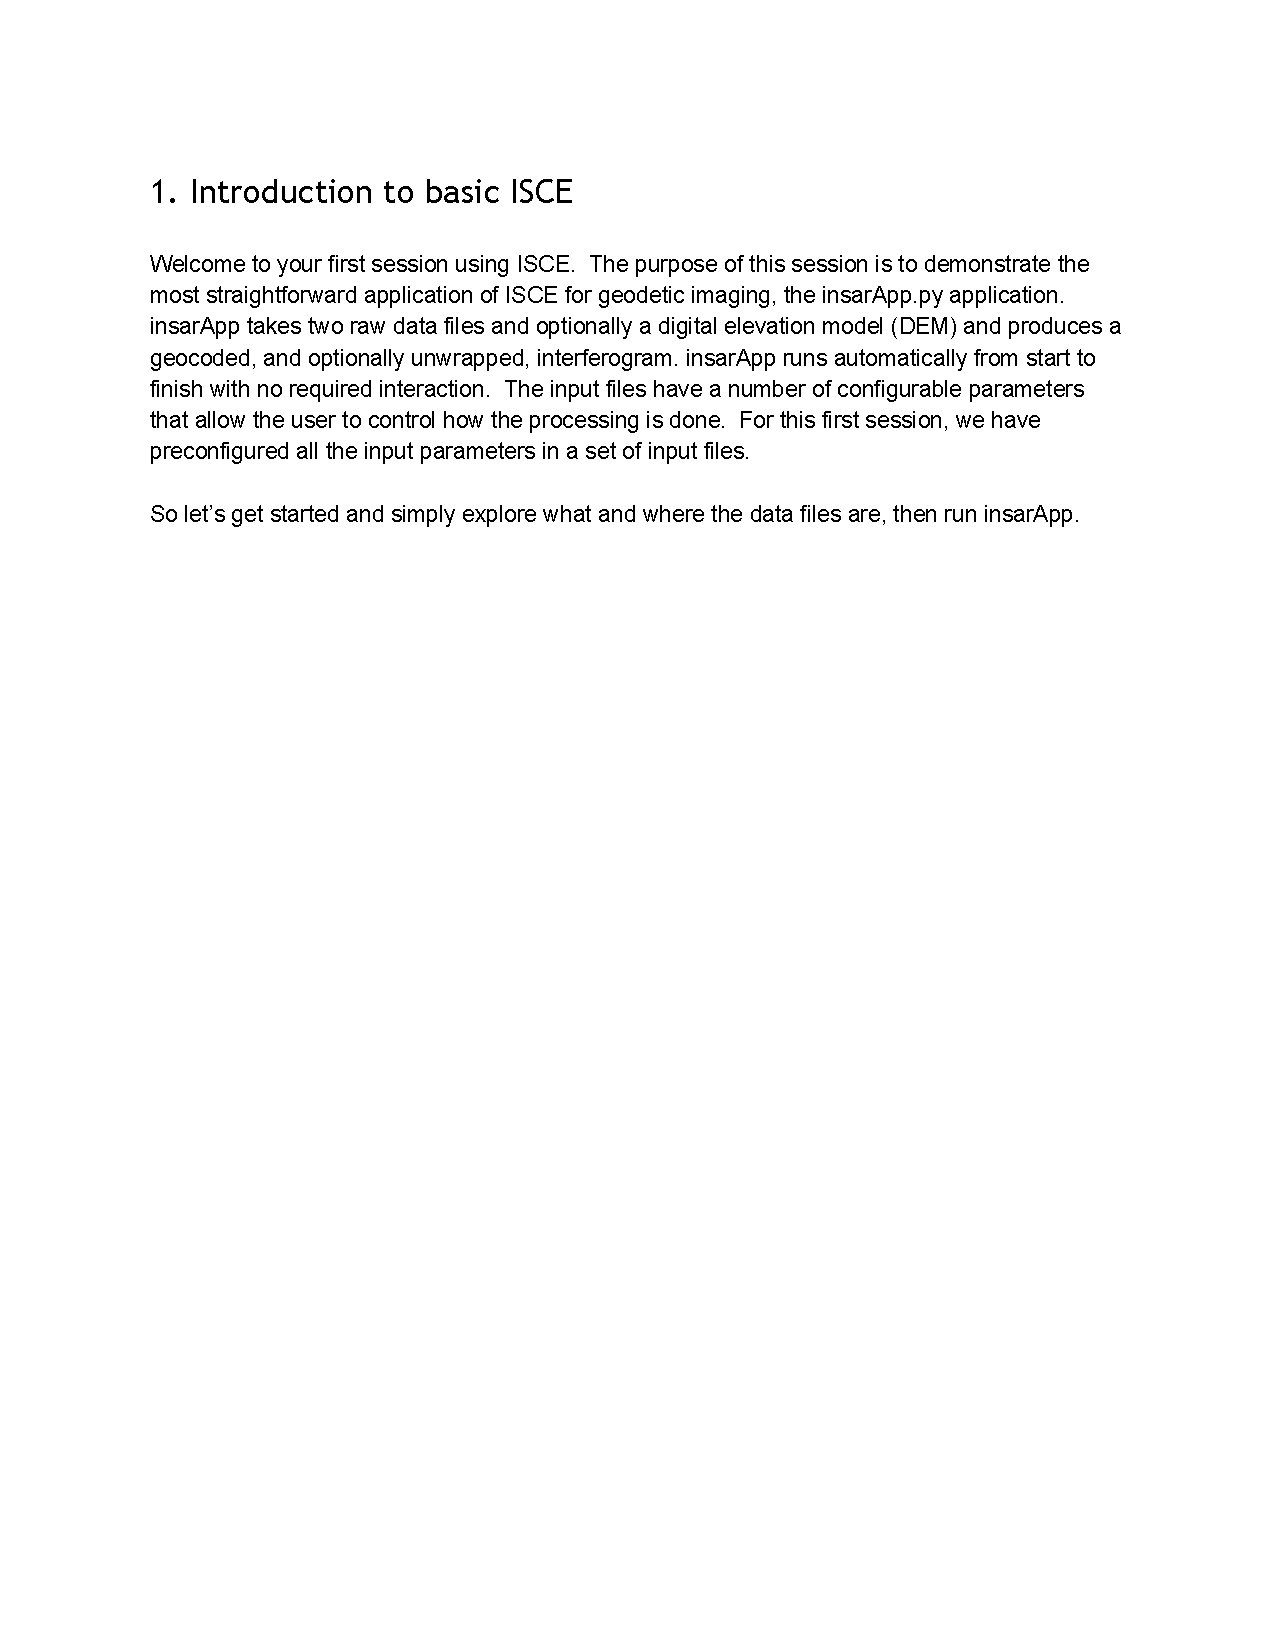
\includepdf[pages=-]{Lab1GettingstartedwithISCE.pdf}
\includepdf[pages=-]{Lab1_1NumberFormatsinISCE.pdf}

\chapter{Using MDX}
\includepdf[pages=-]{Lab2UsingMDX.pdf}

\chapter{Processing Interferometric Data Sets Using insarApp.py}
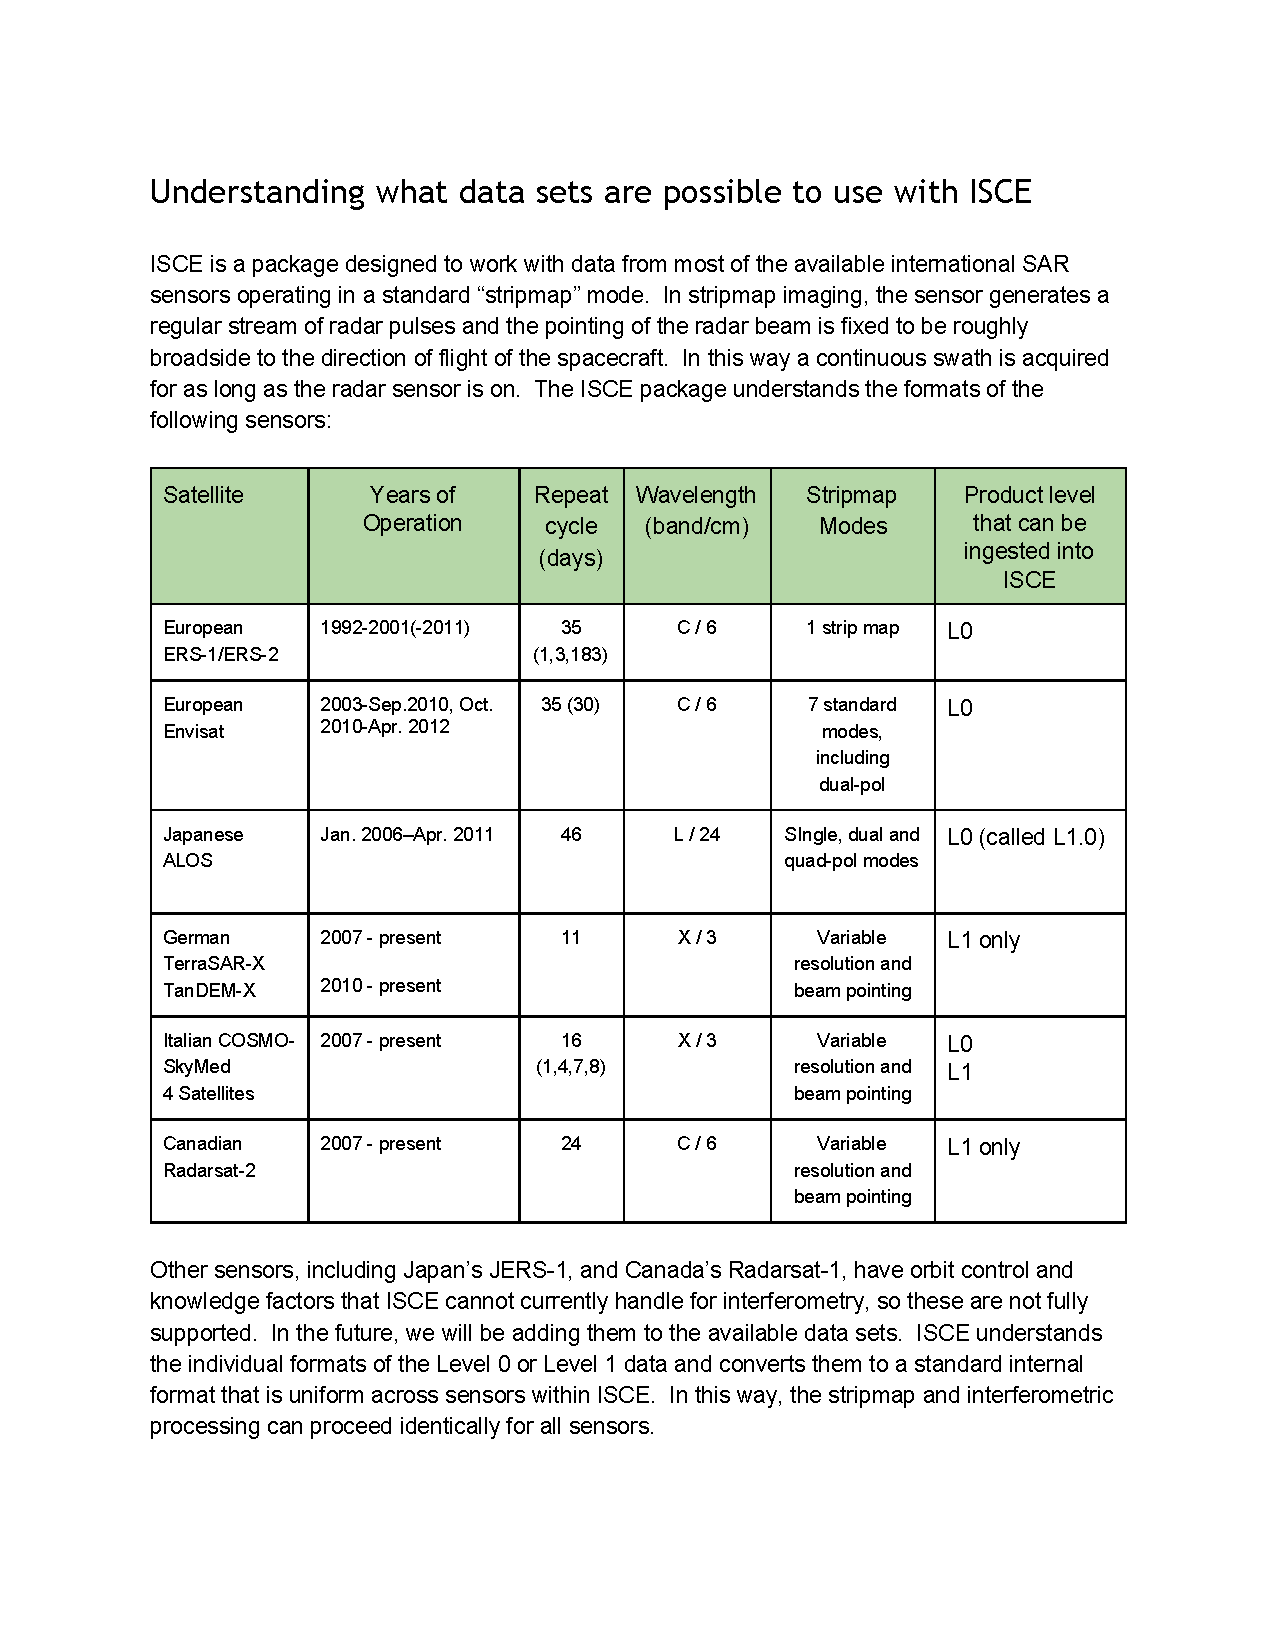
\includepdf[pages=-]{Lab3_0ProcessingInterferometricDataSetsusinginsarApp_Overview.pdf}
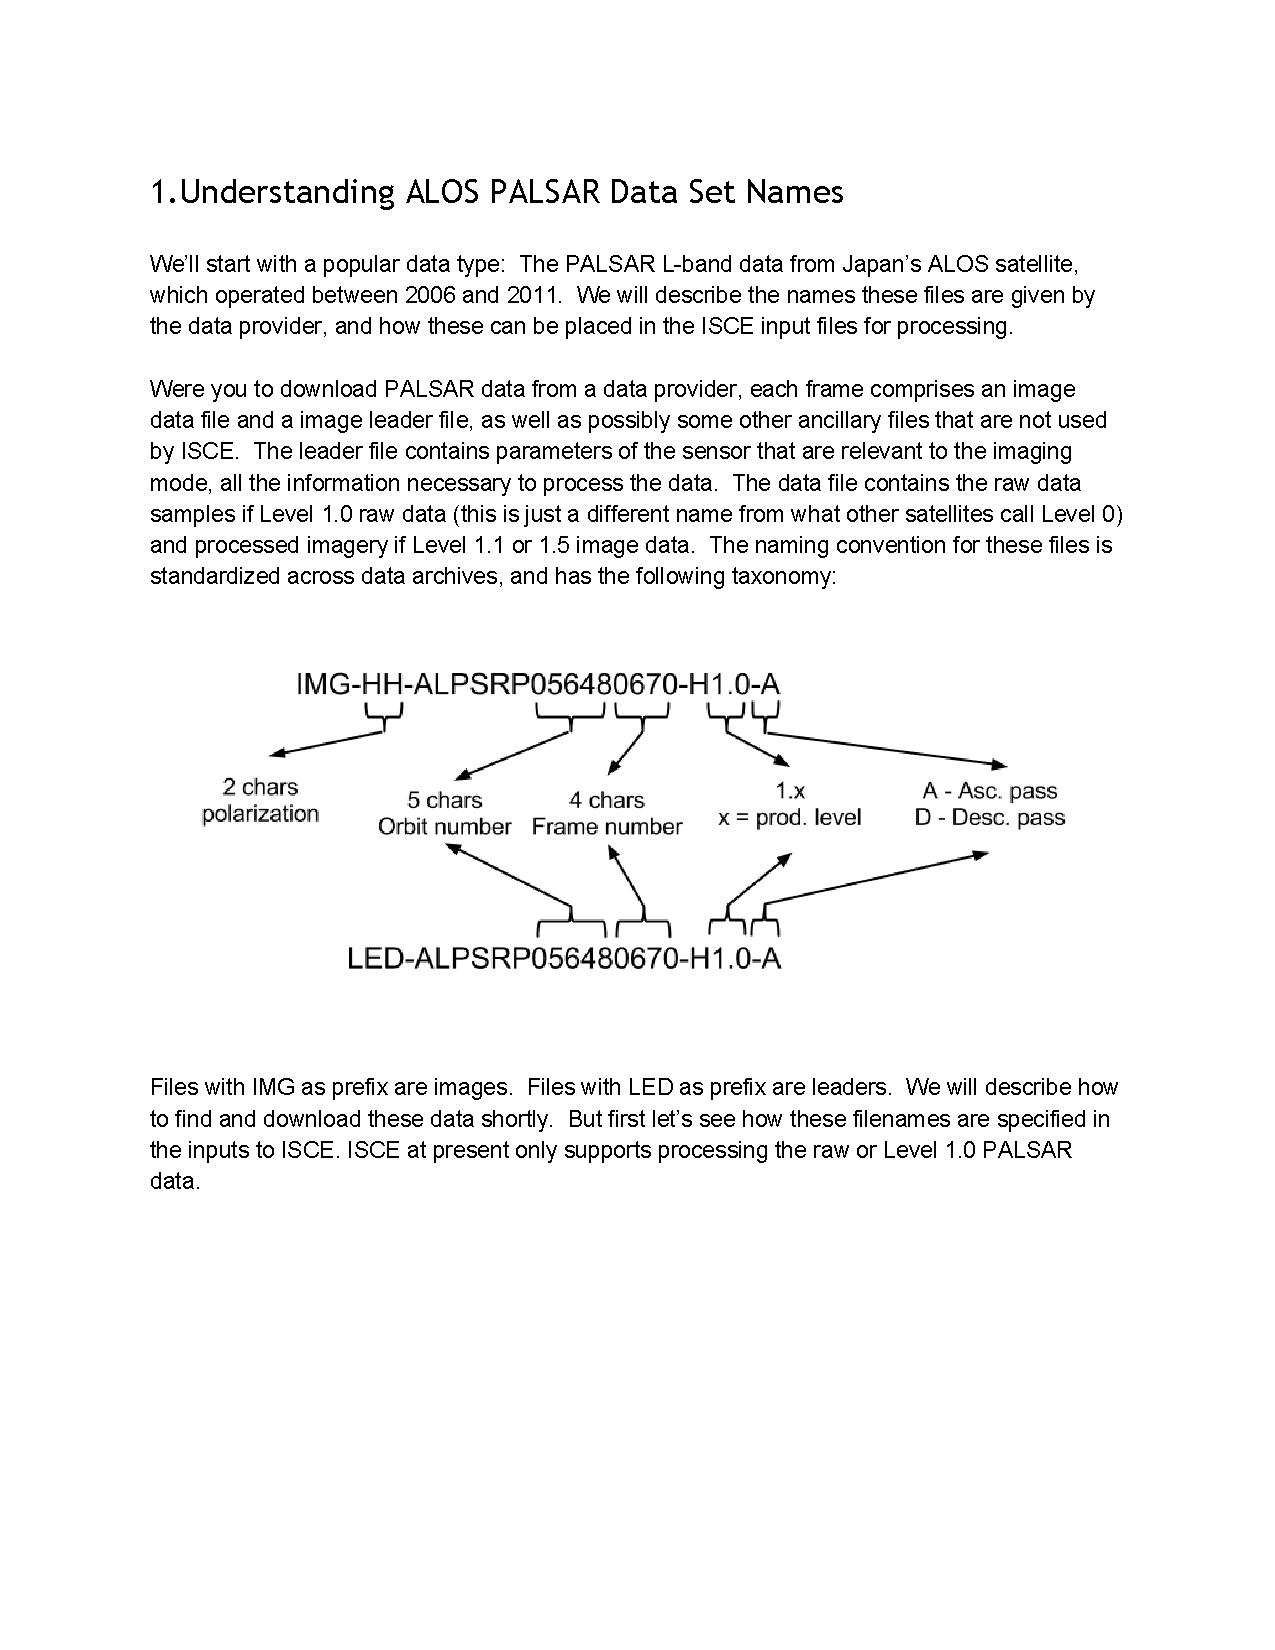
\includepdf[pages=-]{Lab3_1ProcessingALOSPALSAR.pdf}
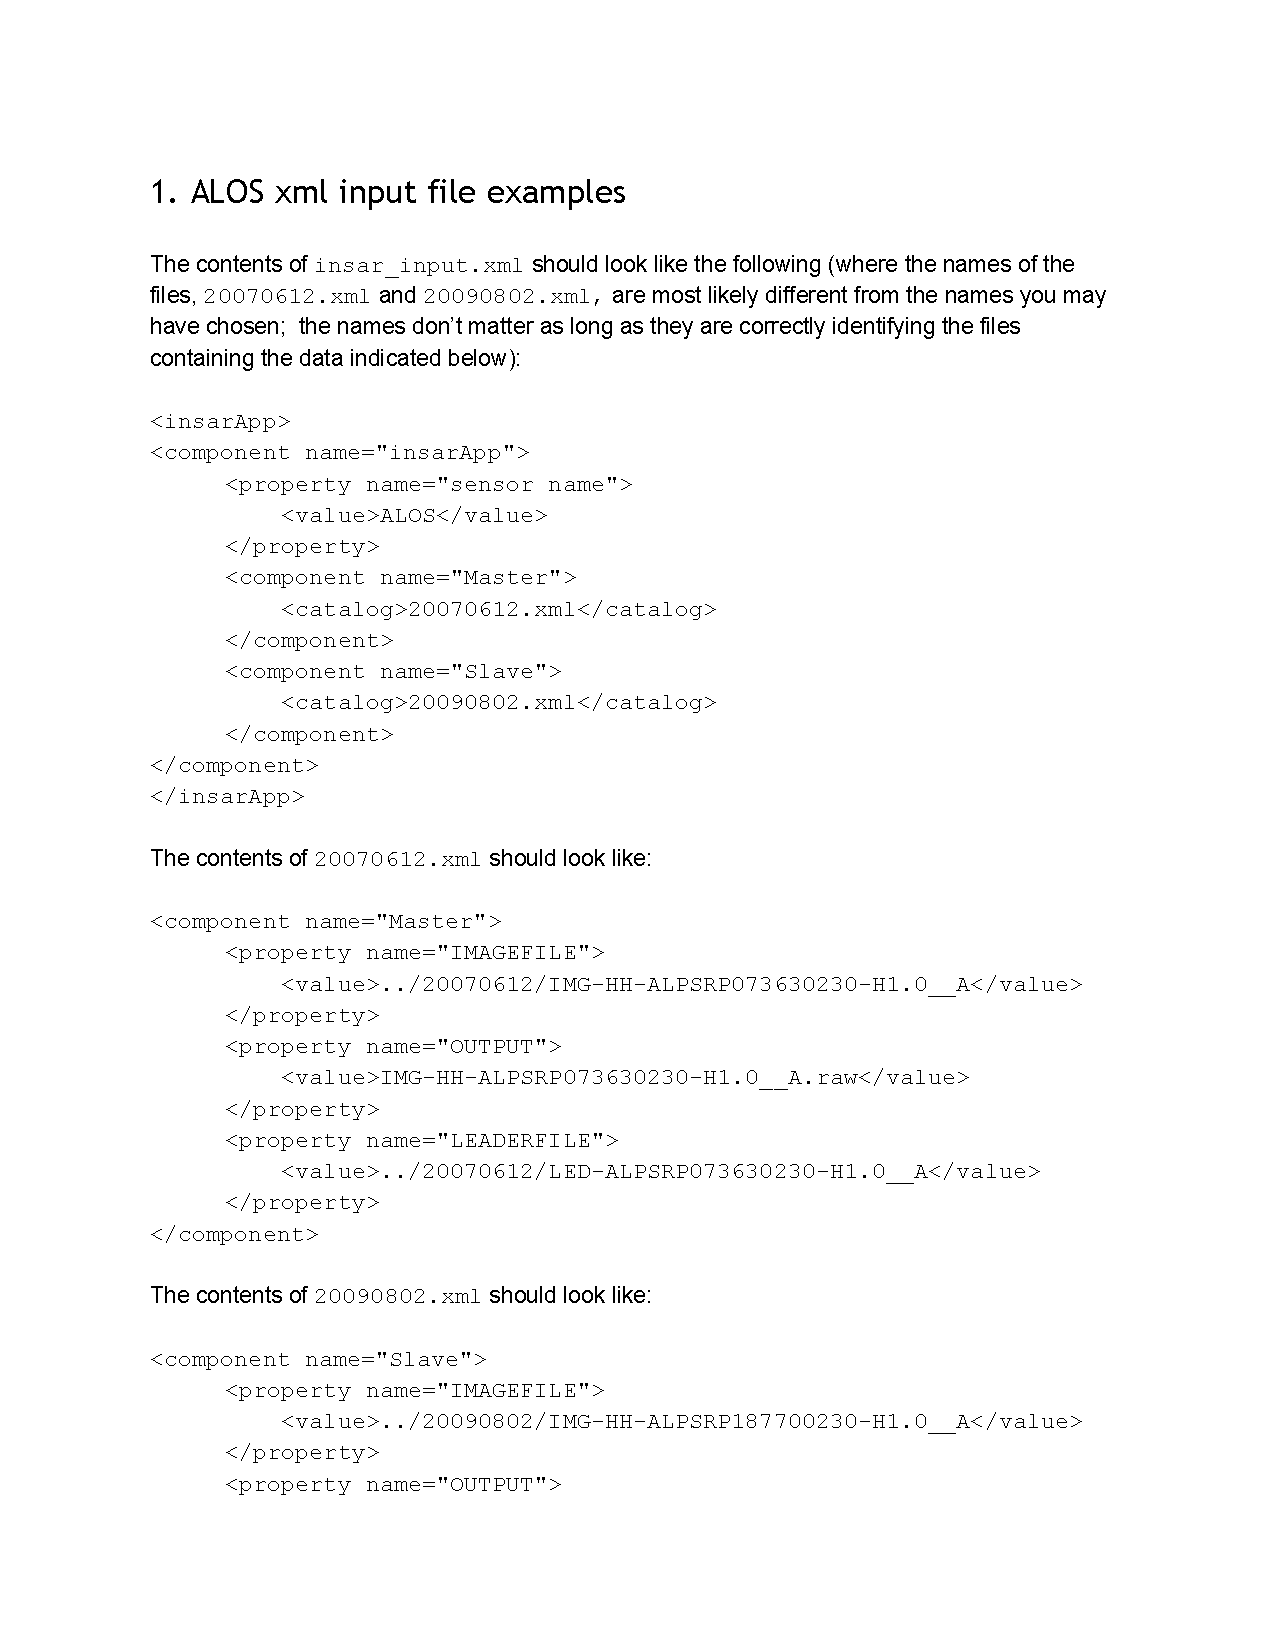
\includepdf[pages=-]{Lab3_1_1ALOSxmlinputfileexamples.pdf}
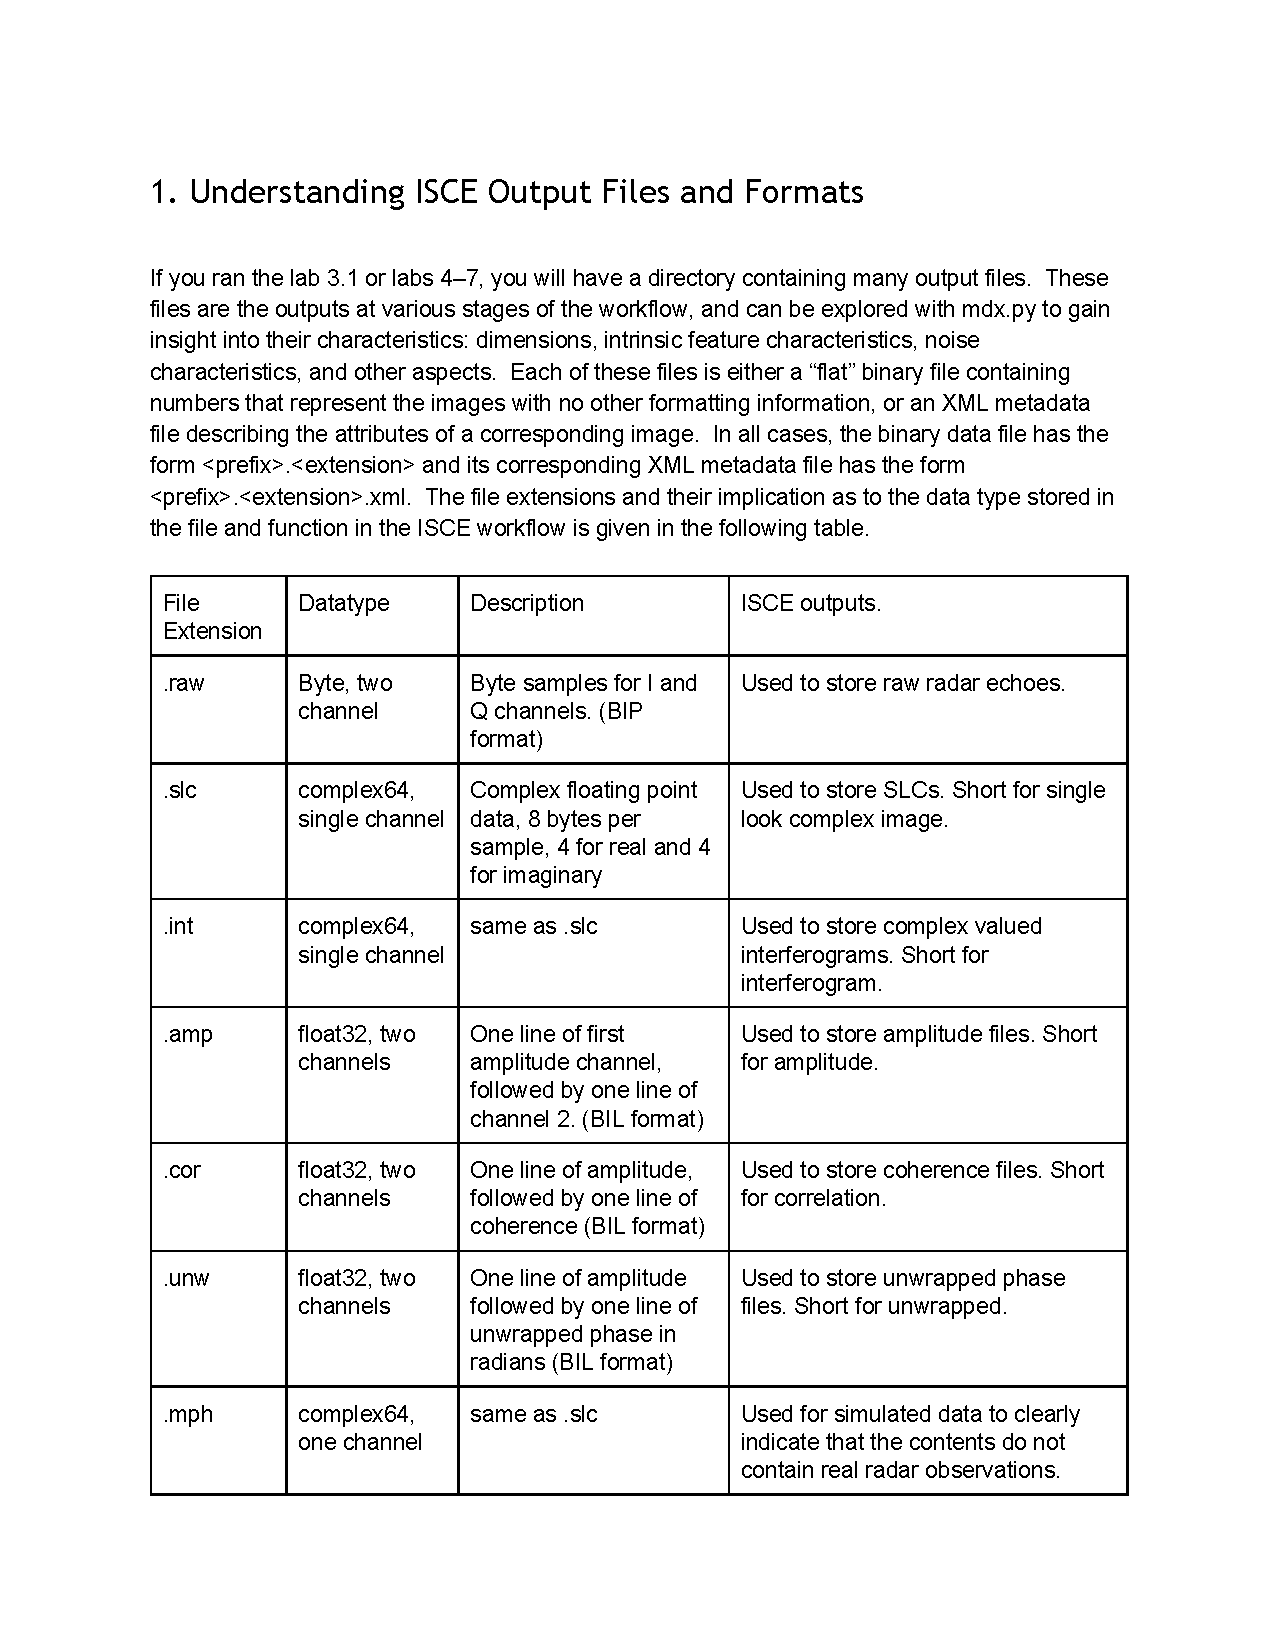
\includepdf[pages=-]{Lab3_2UnderstandingOutputFilesandFormats.pdf}
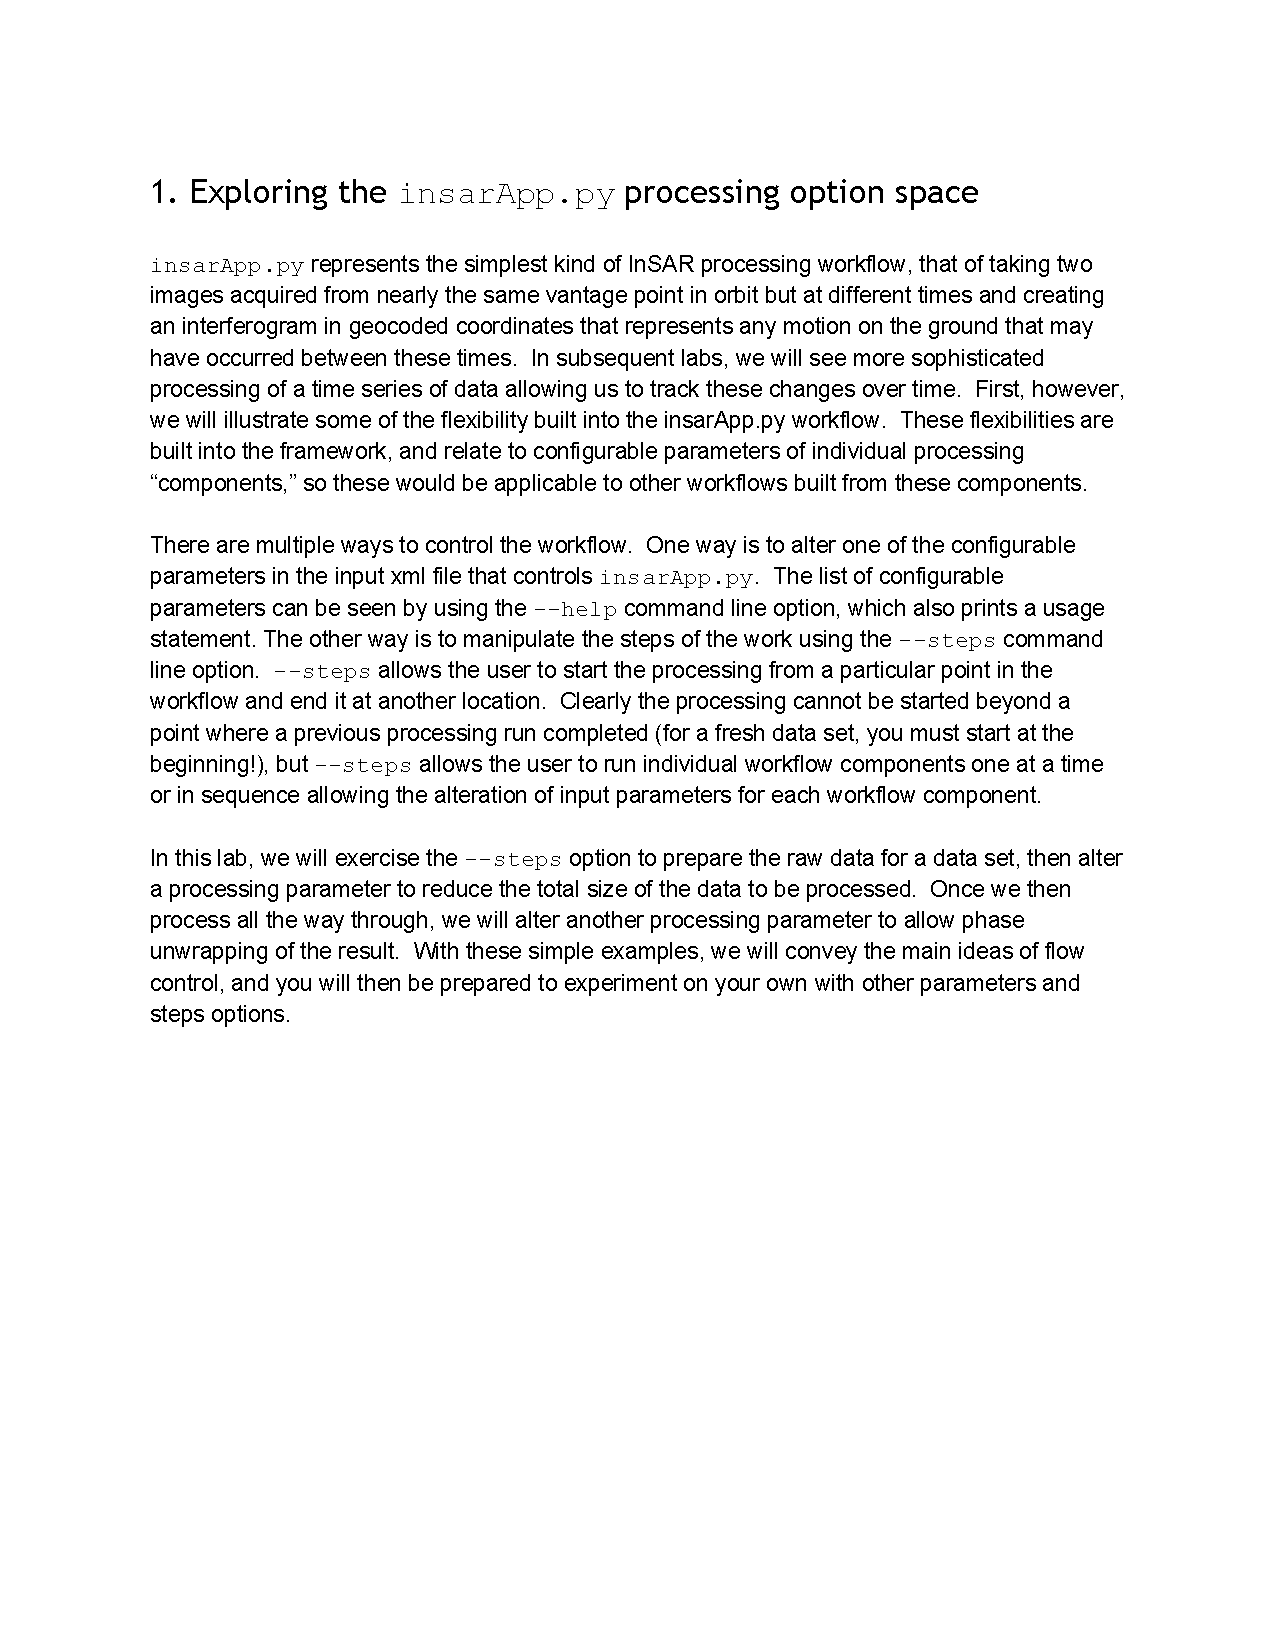
\includepdf[pages=-]{Lab3_3ExploringtheinsarAppprocessingoptionspace.pdf}
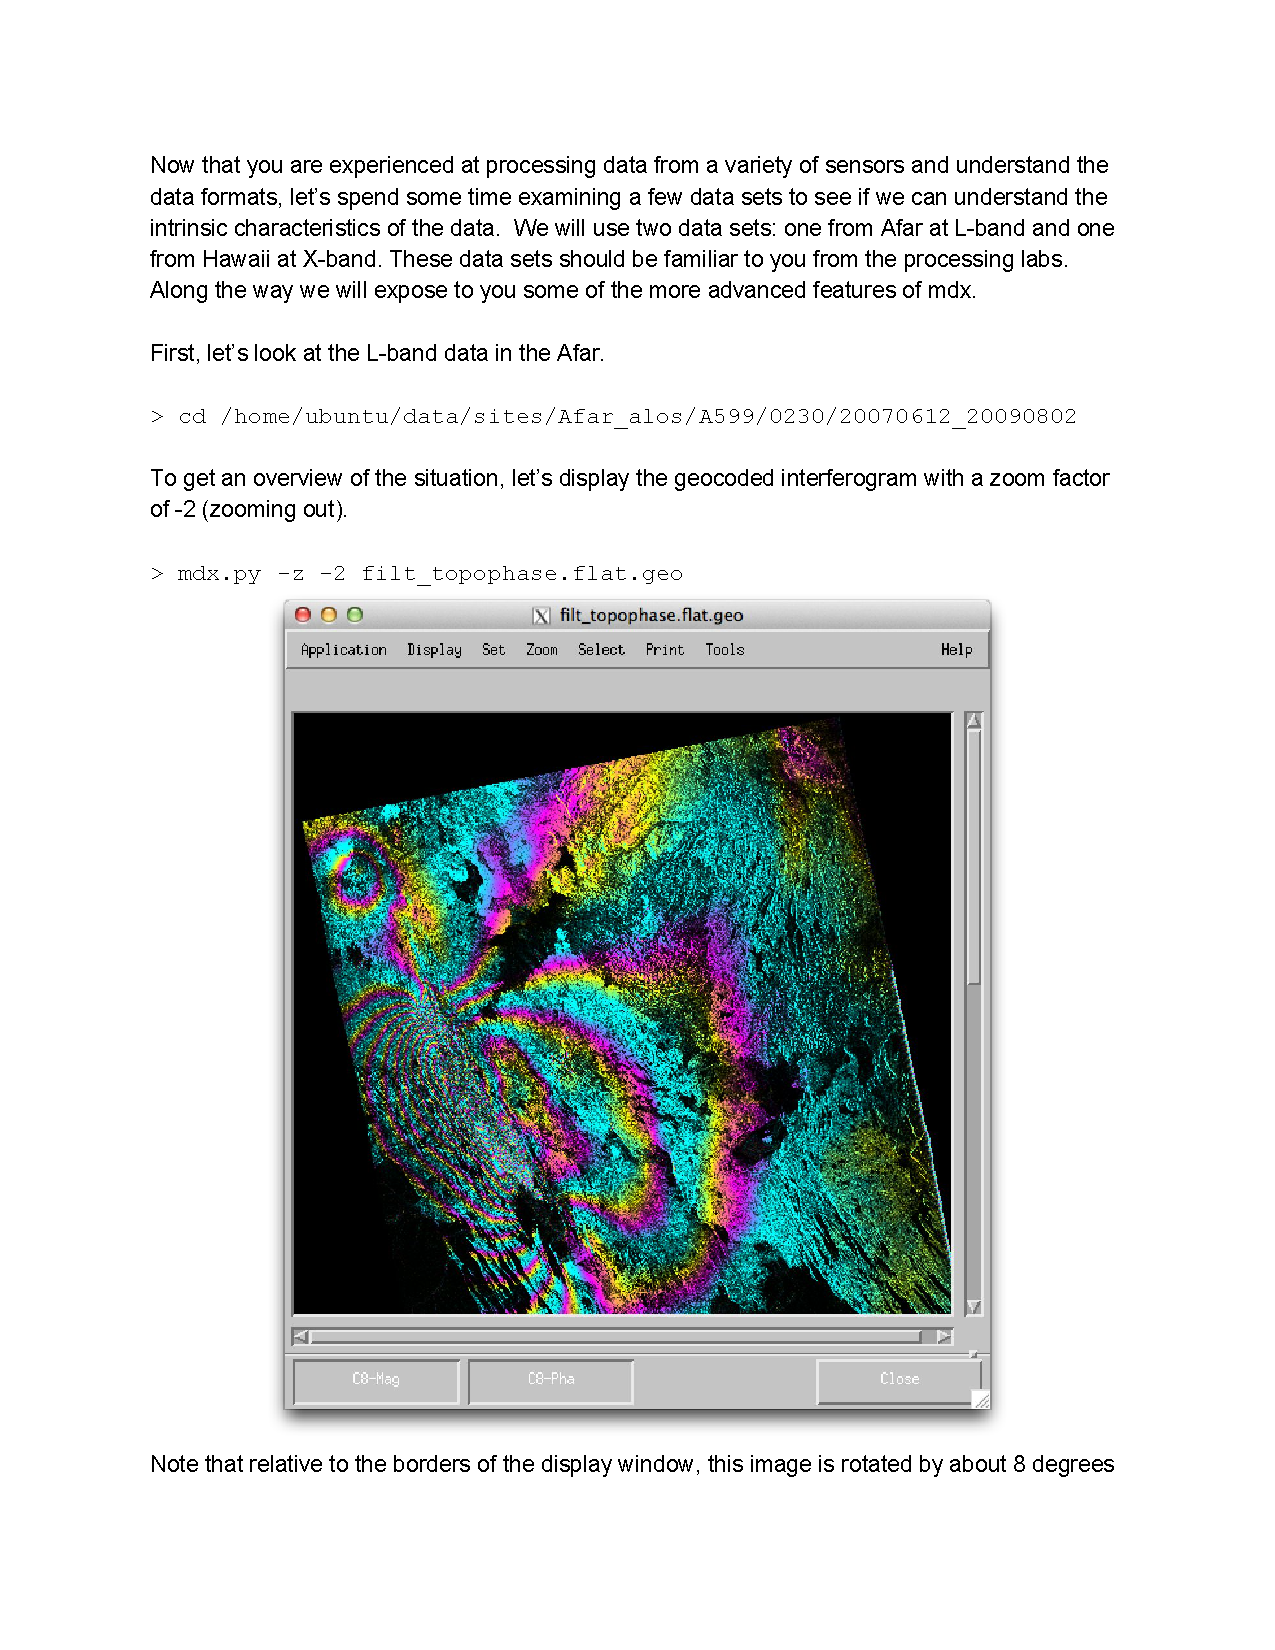
\includepdf[pages=-]{ExploringInterferometricDataCharacteristics.pdf}

\chapter{Processing ERS Data}
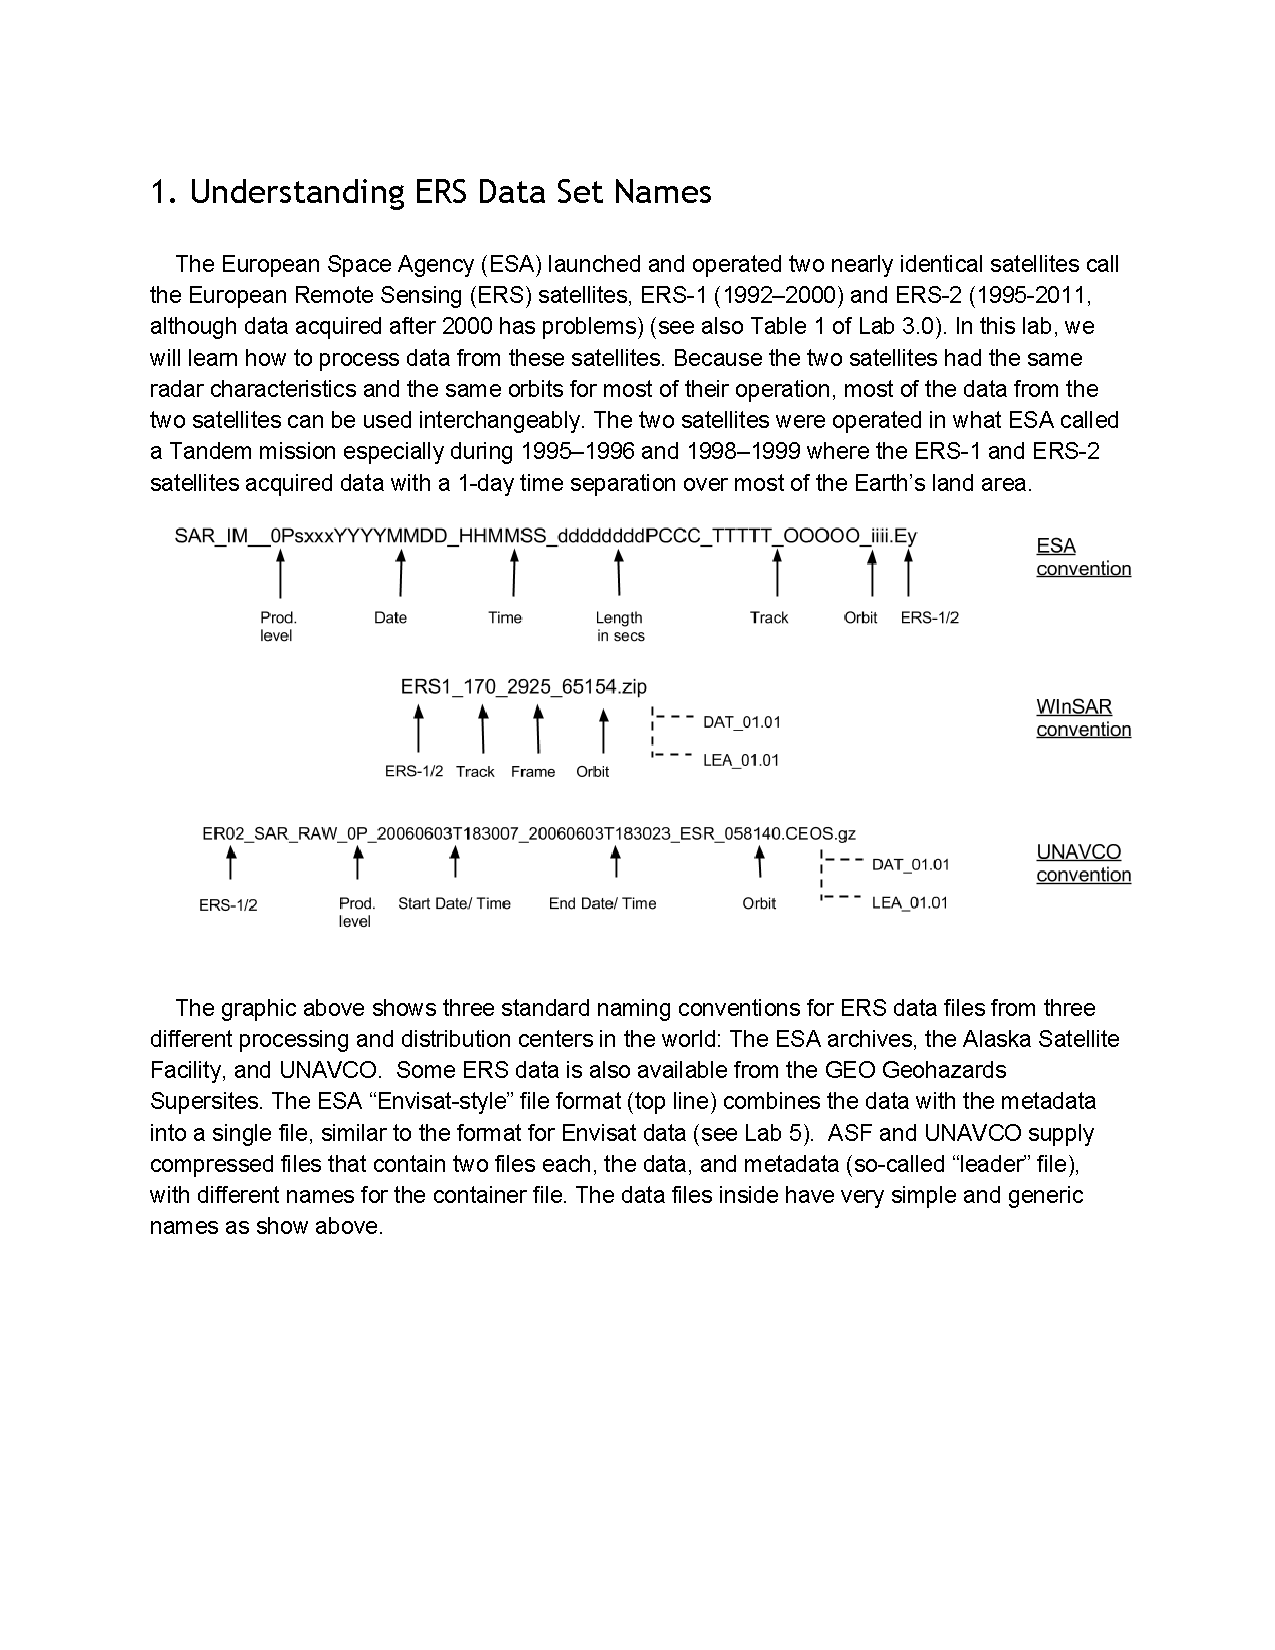
\includepdf[pages=-]{Lab4_0ProcessingERS.pdf}
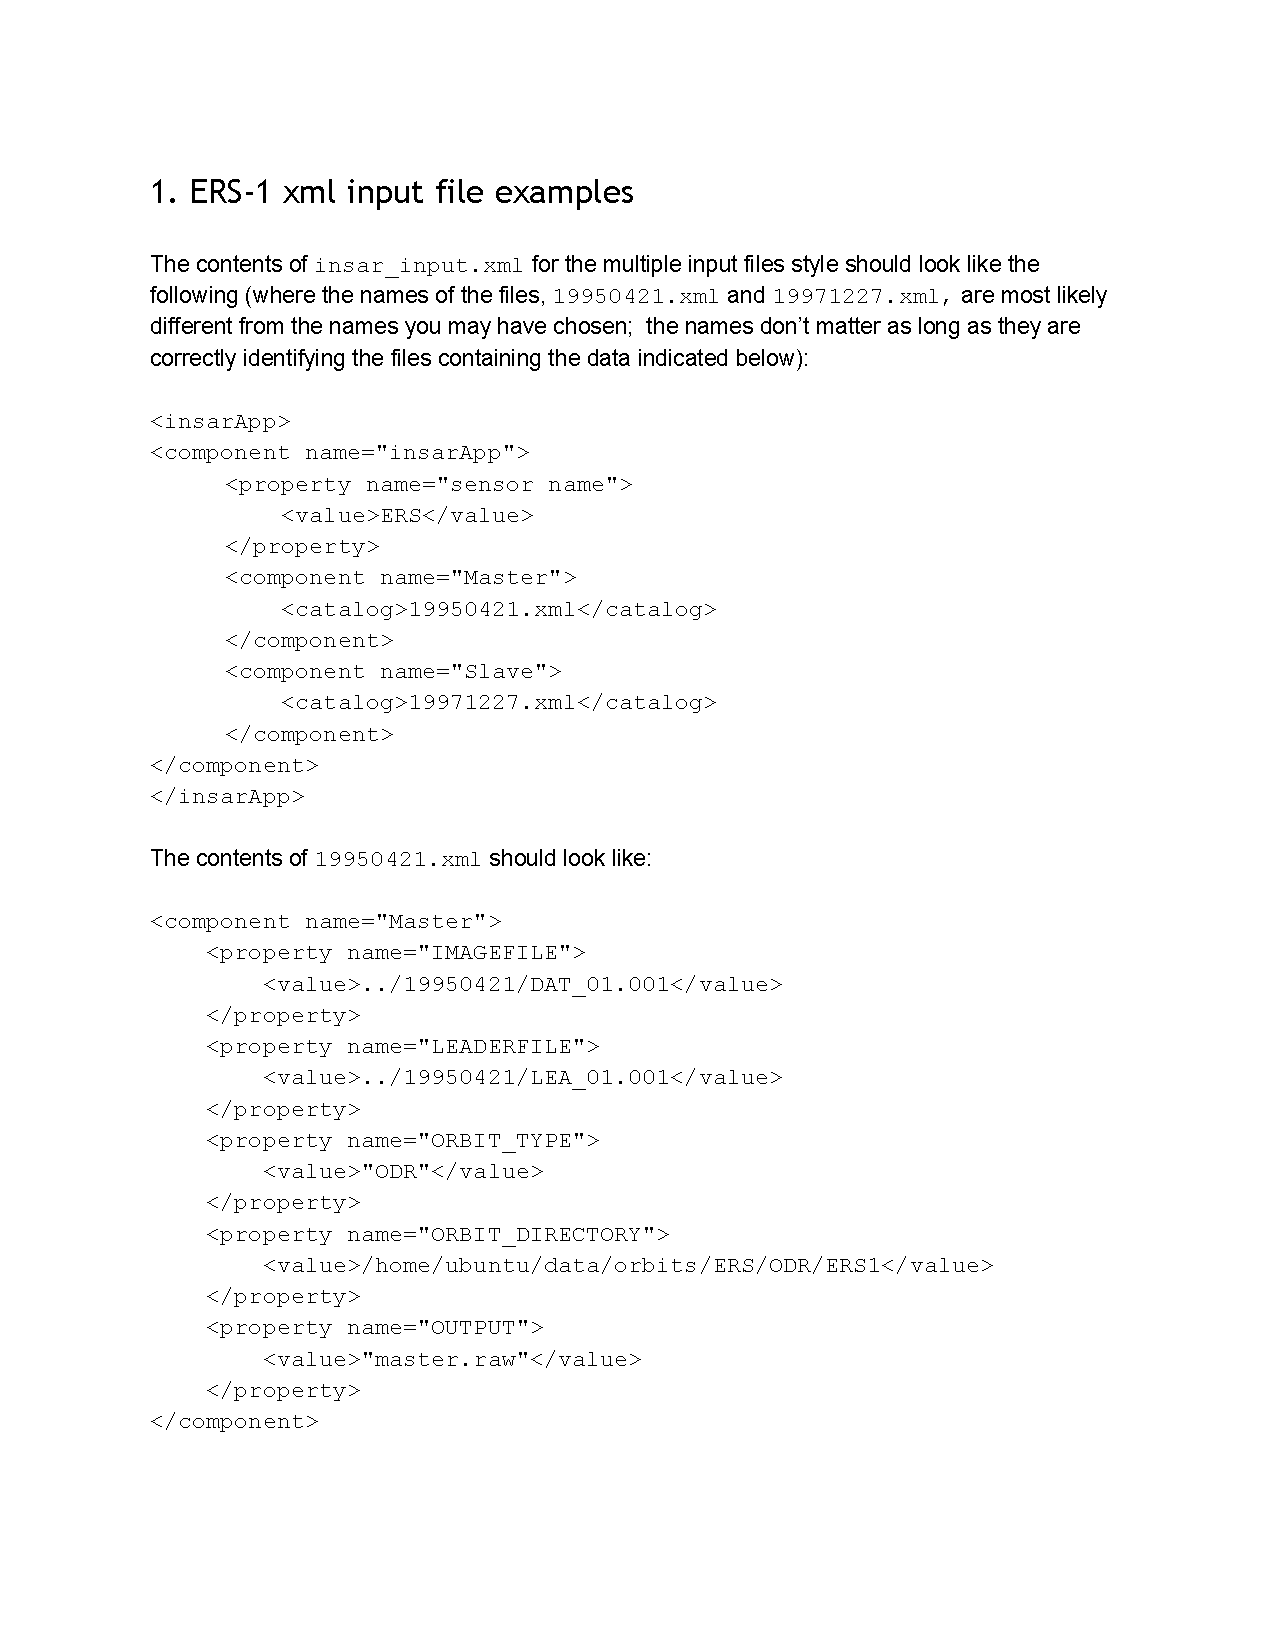
\includepdf[pages=-]{Lab4_1ERSxmlinputfileexamples.pdf}

\chapter{Processing Envisat Data}
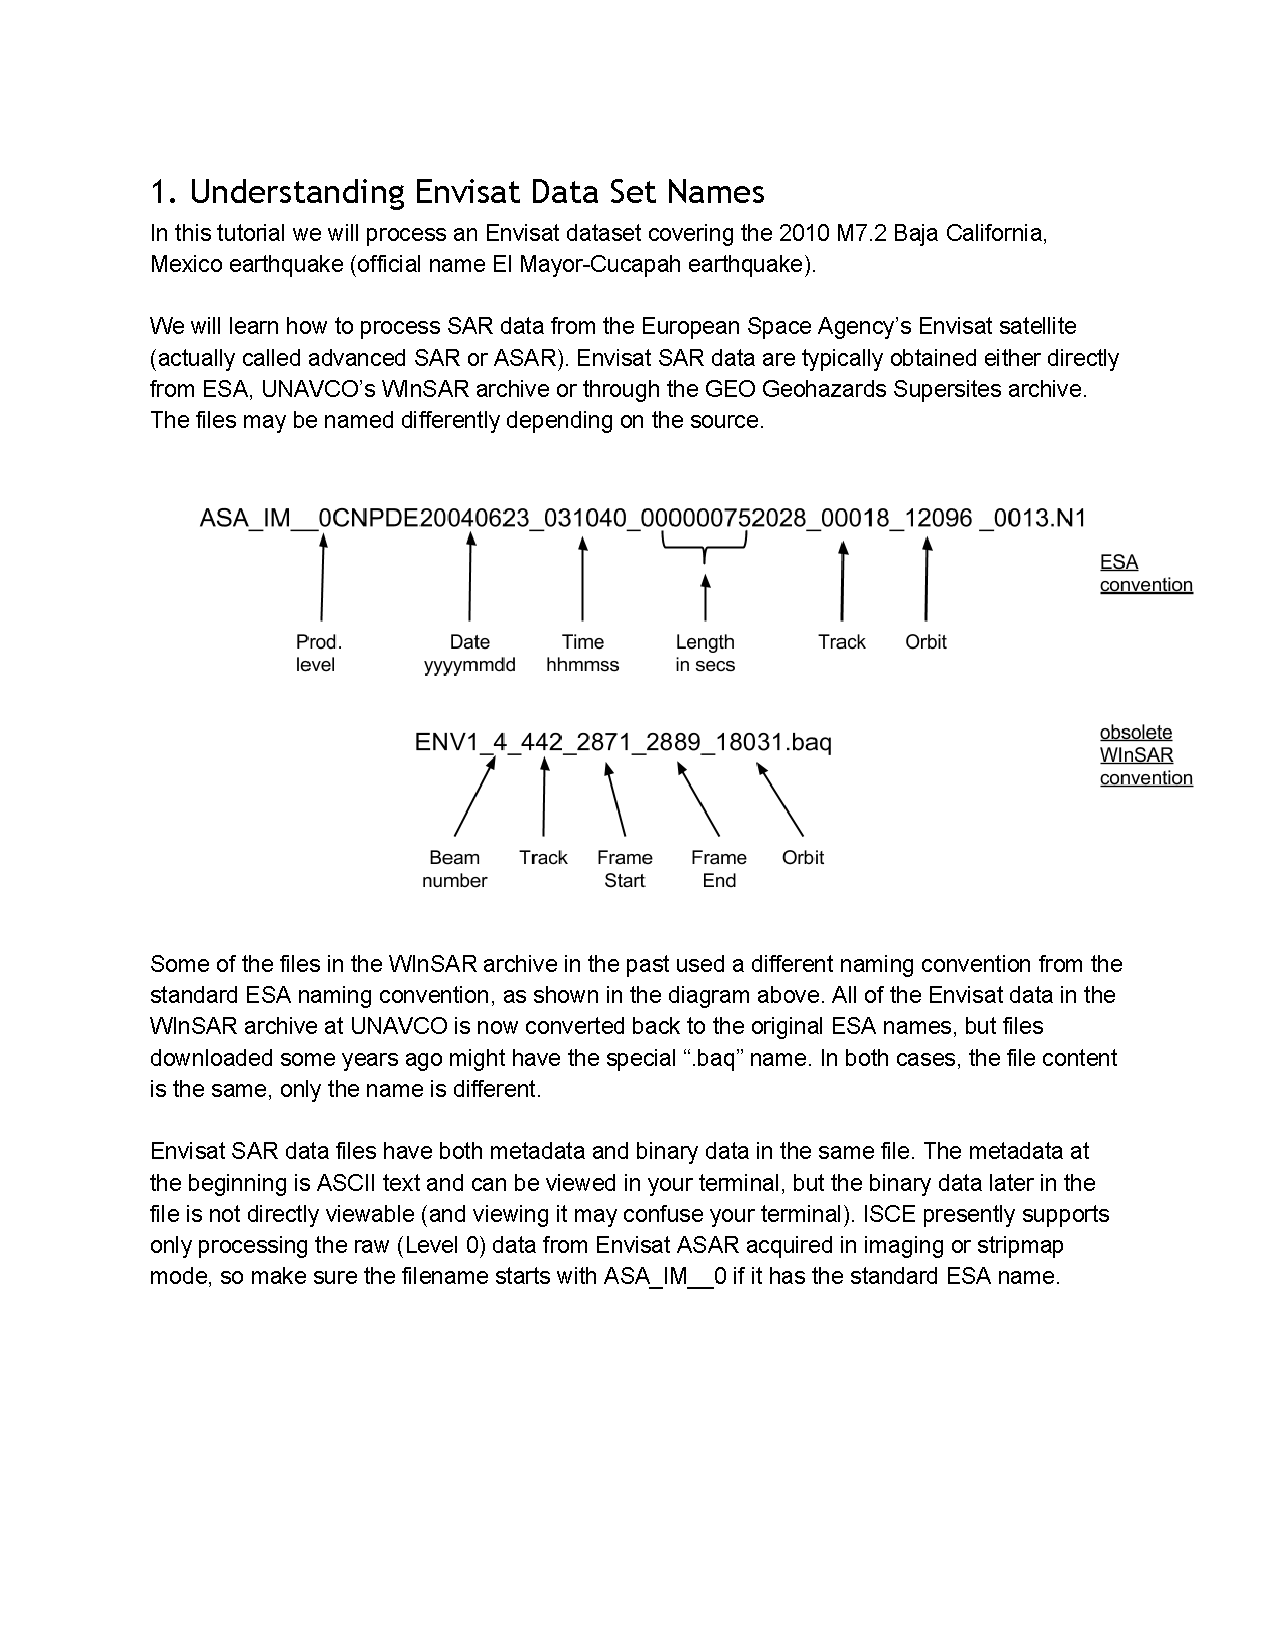
\includepdf[pages=-]{Lab5ProcessingEnvisat.pdf}

\chapter{Processing COSMO-SkyMed Raw Data}
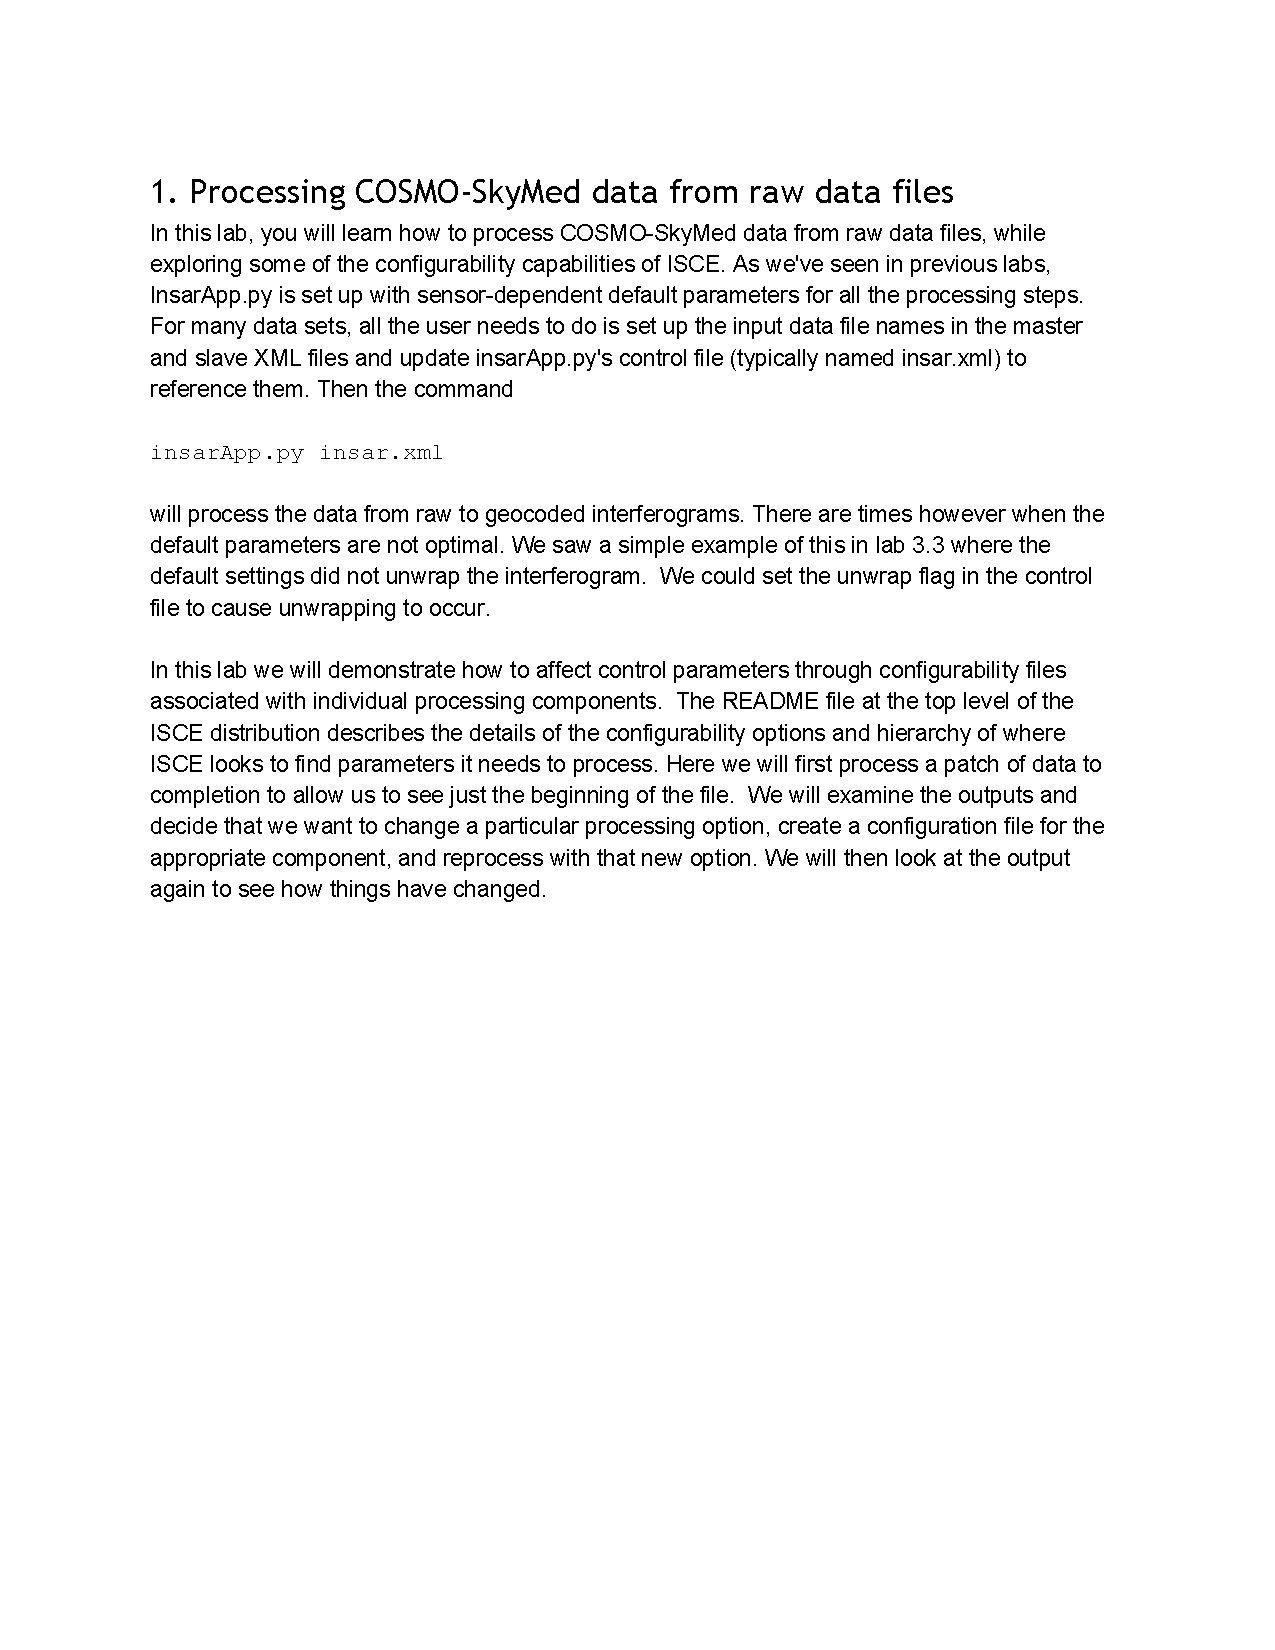
\includepdf[pages=-]{Lab6ProcessingCOSMO-SkyMedrawdataISCEconfigurationoptions.pdf}

\chapter{Processing From SLC: COSMO-SkyMed, TerraSAR-X, RadarSAT-2, and others}
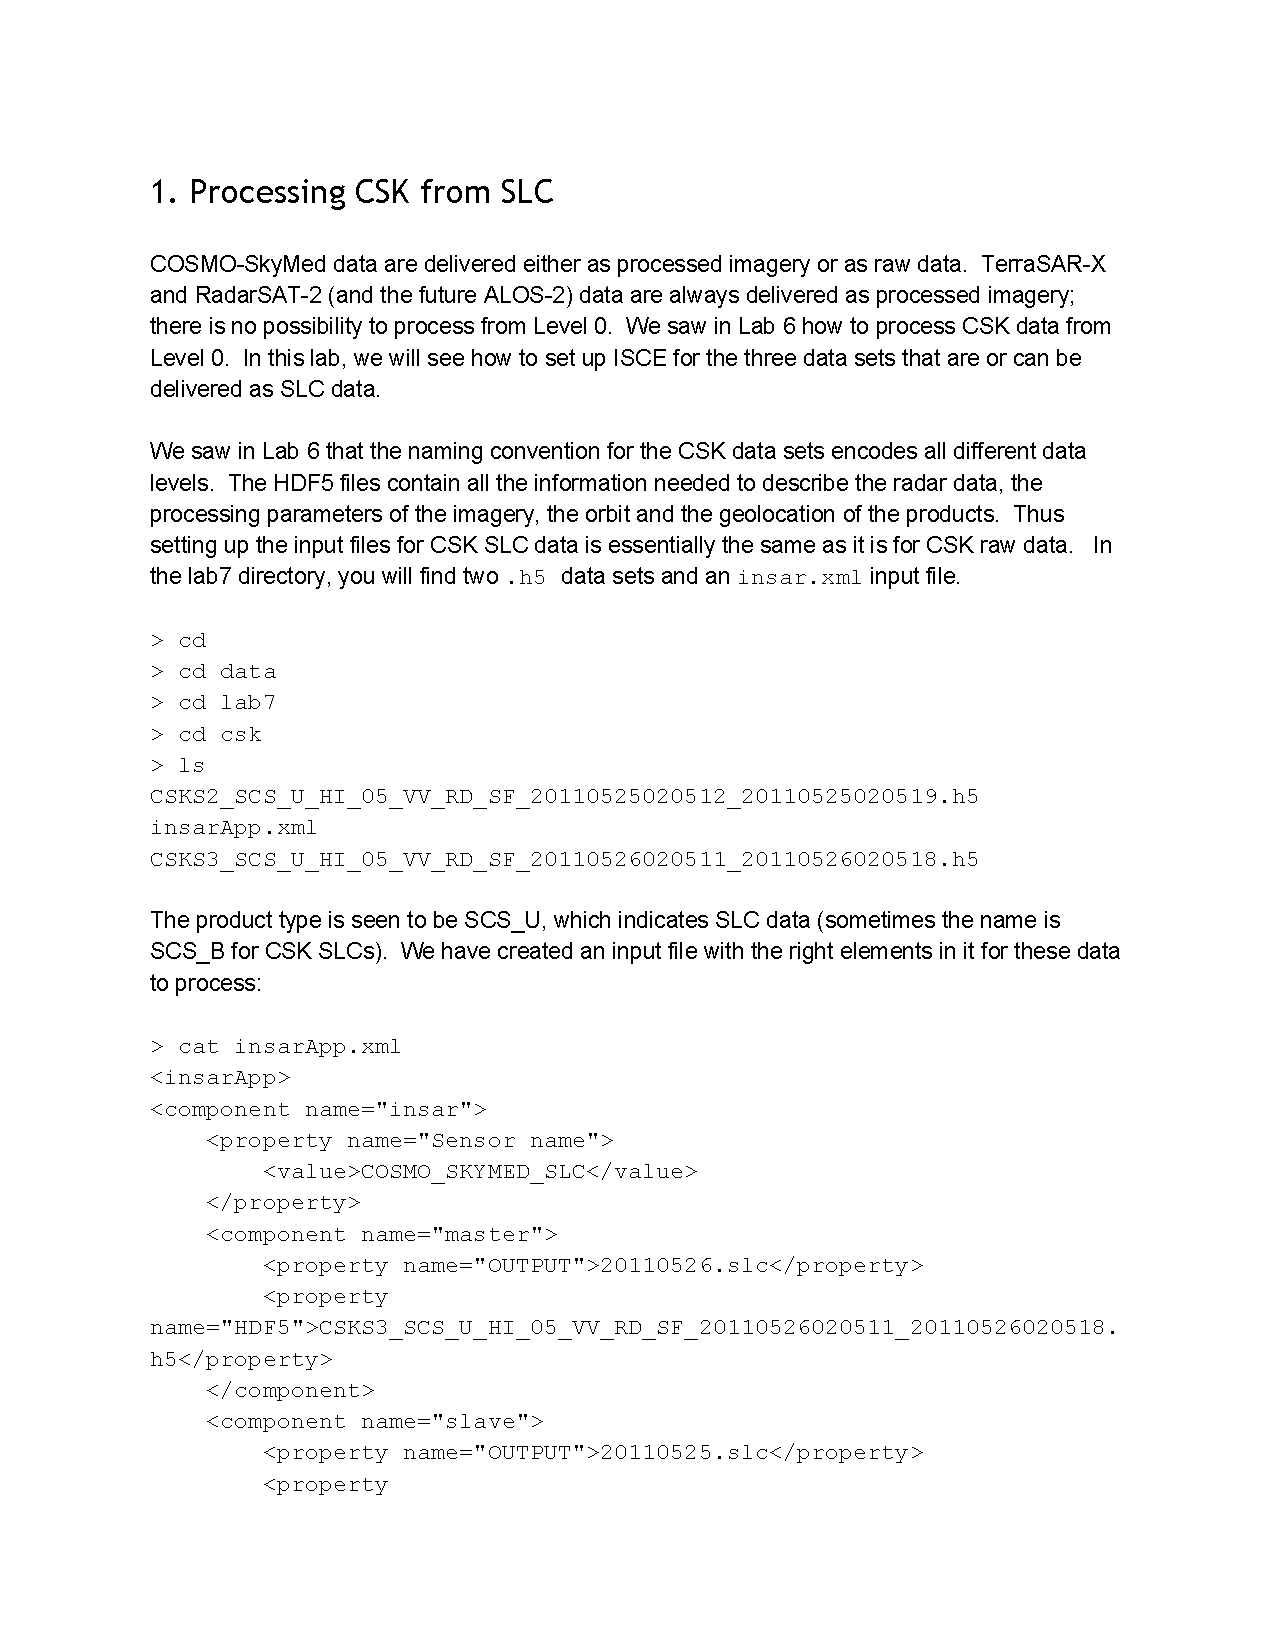
\includepdf[pages=-]{Lab7ProcessingfromSLCCOSMO-SkyMedTerraSAR-XRadarSAT-2andothers.pdf}

\chapter{ISCE Stack Processing for GIAnT}
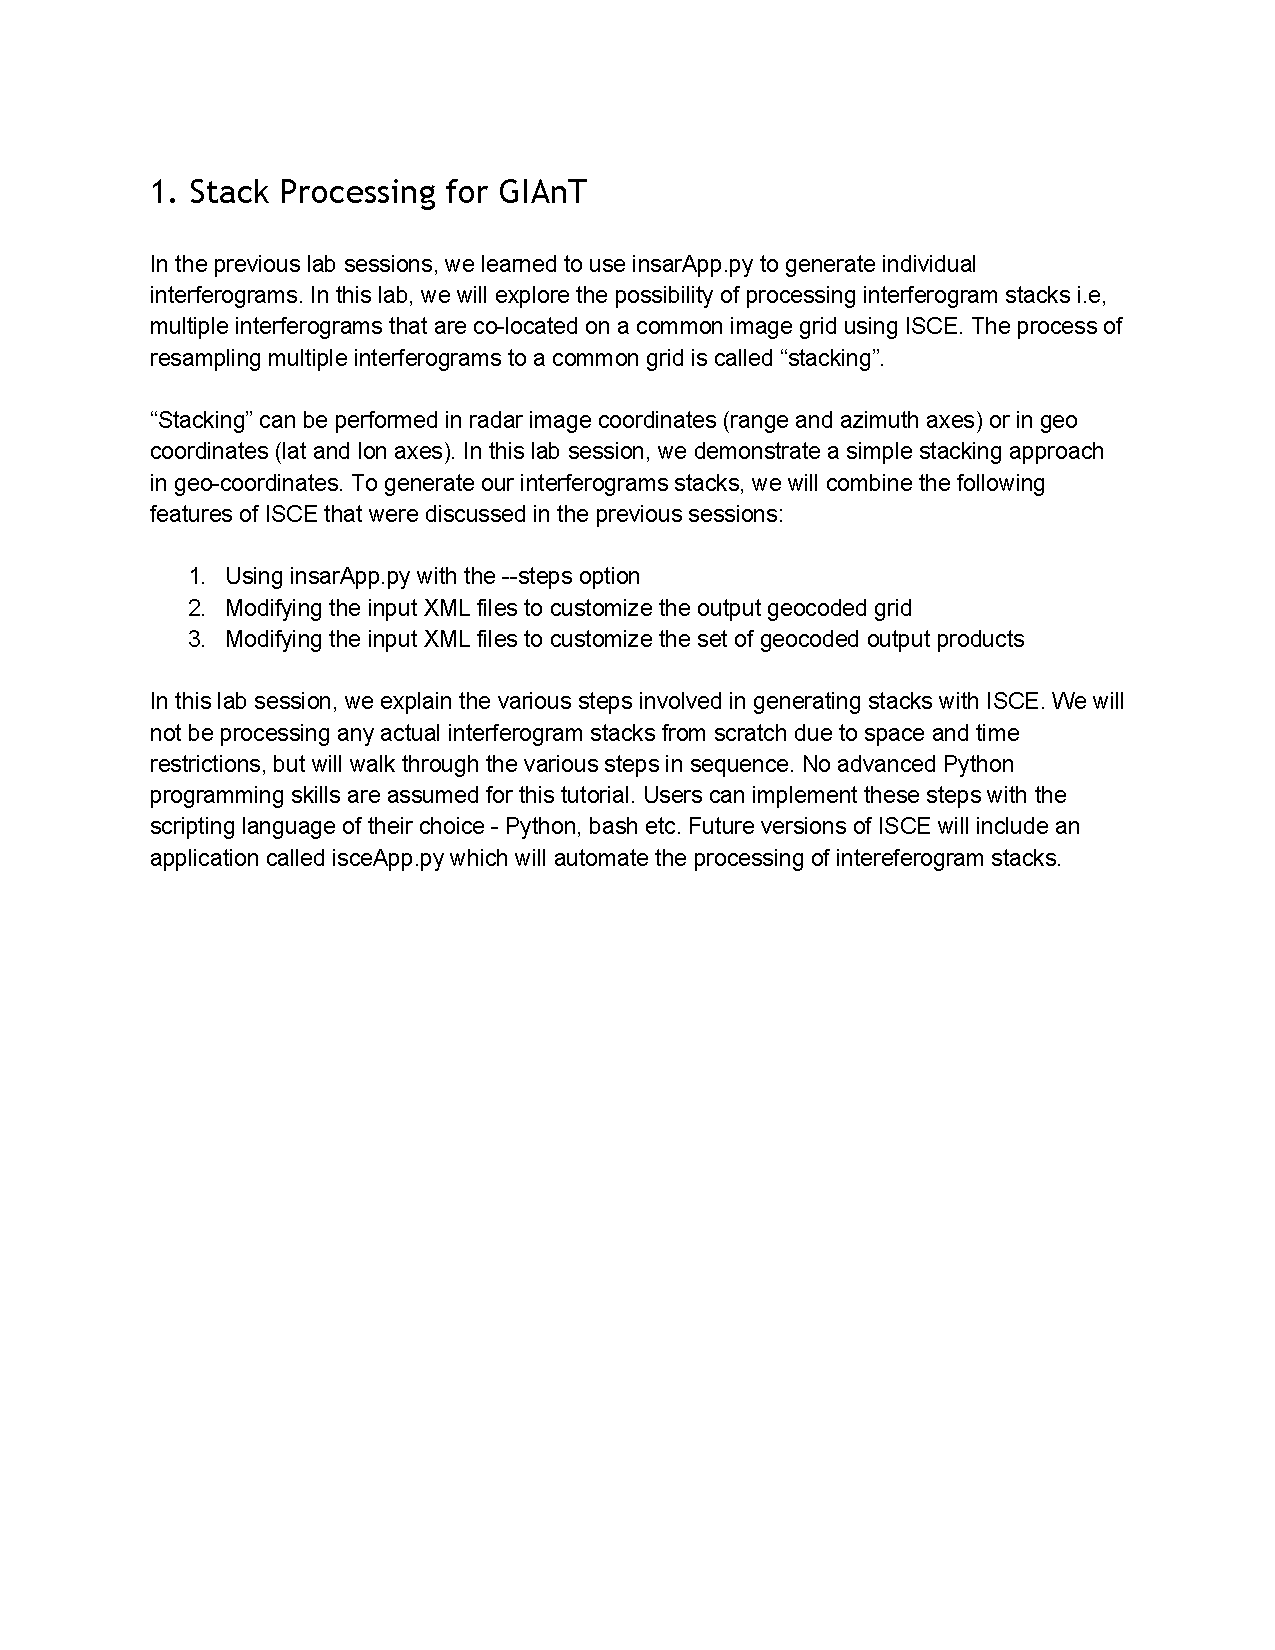
\includepdf[pages=-]{Lab8ISCEStackProcessingforGIAnT.pdf}

\chapter{Working with GIAnT}
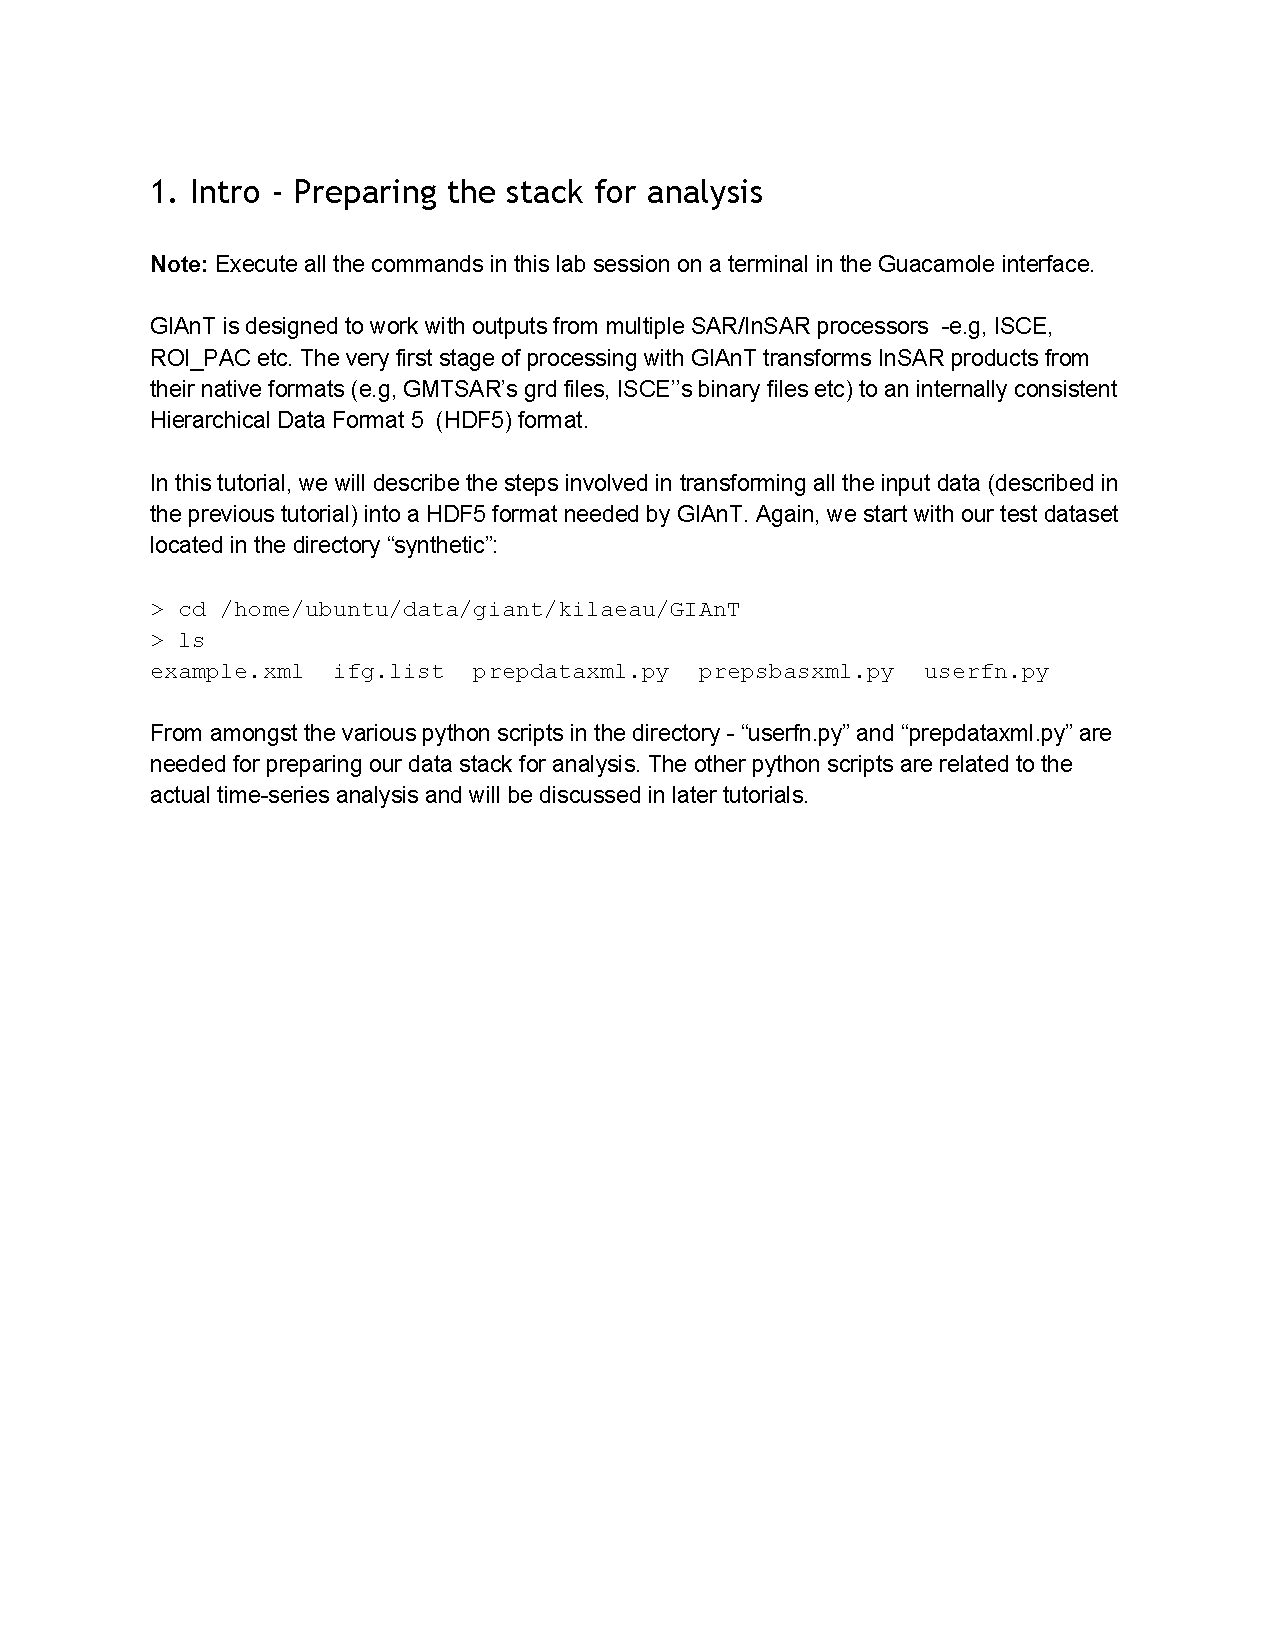
\includepdf[pages=-]{Lab9_1GIAnT_reading_the_stack.pdf}
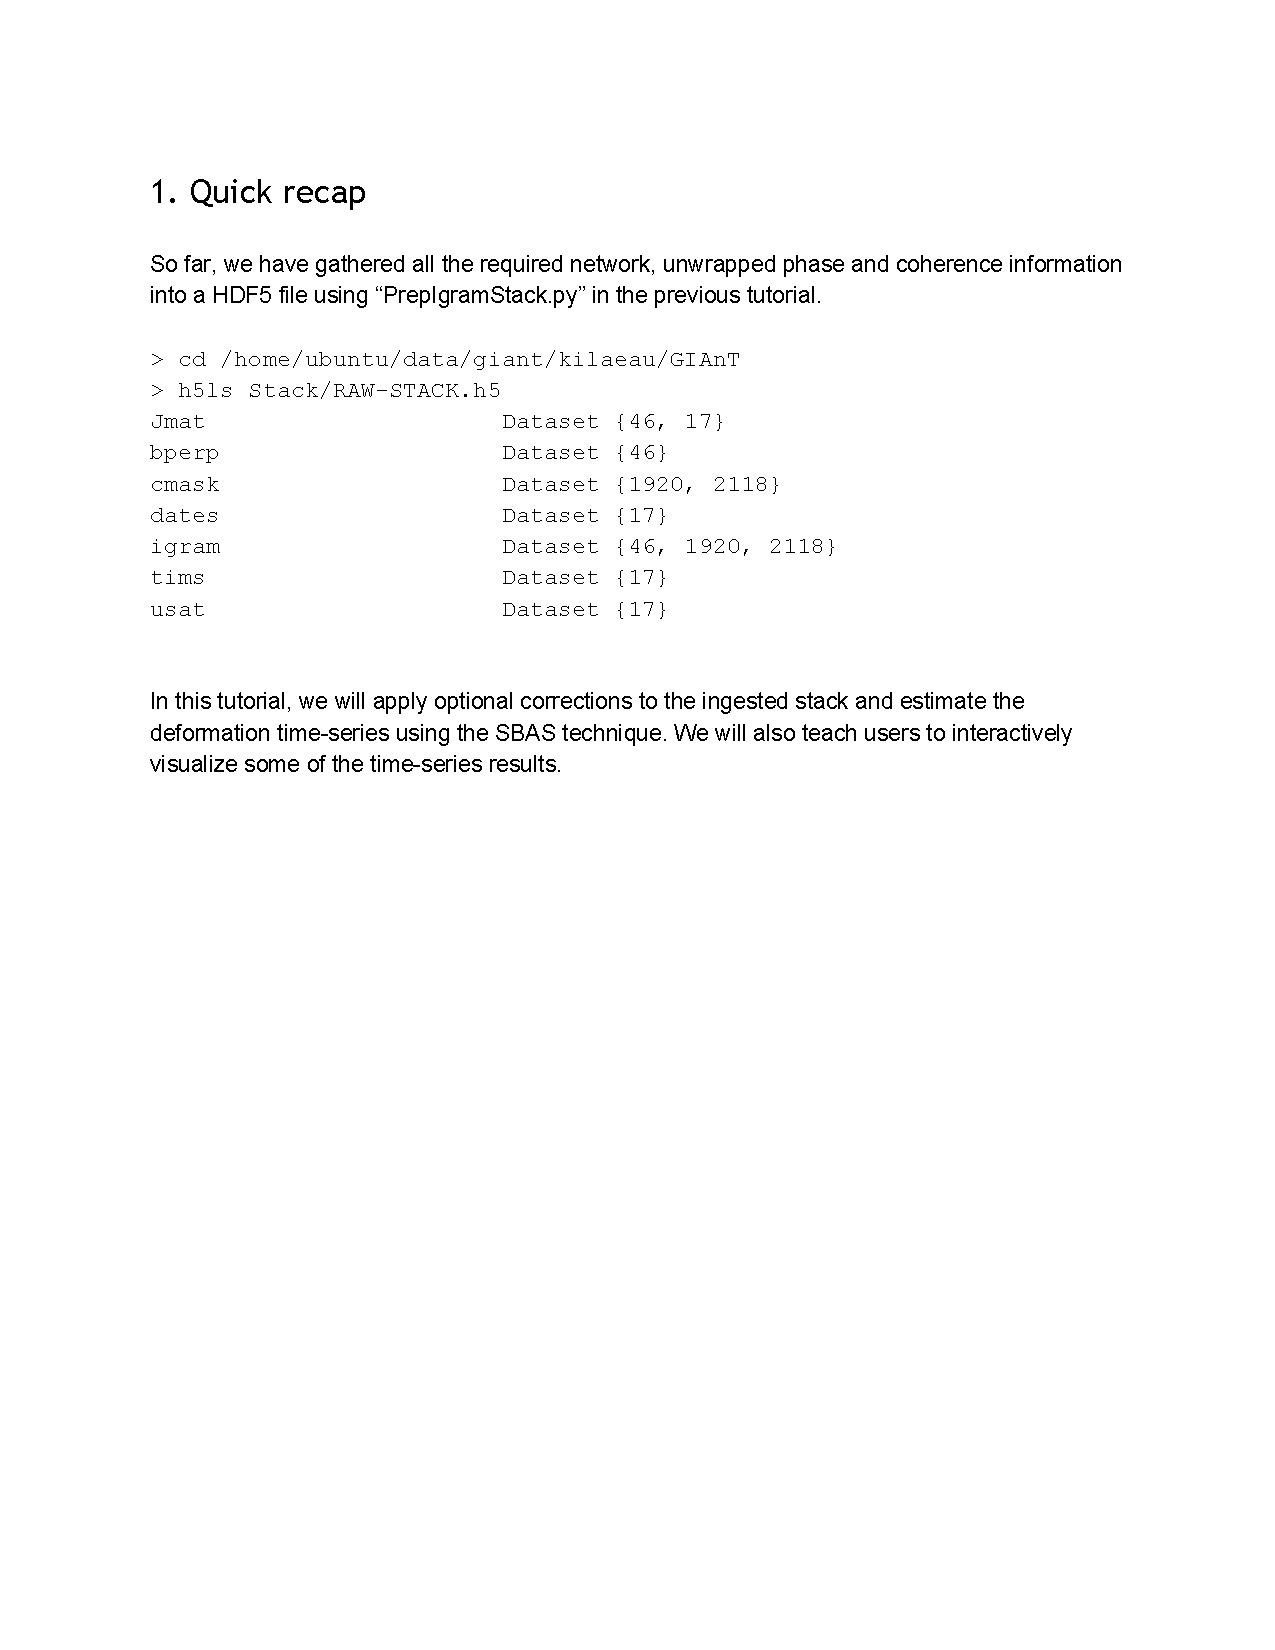
\includepdf[pages=-]{Lab9_2GIAnT_inversion.pdf}

\chapter{Hands On Lab On Polarimetric UAVSAR Data Processing for Land-cover Land-use Change Applications}
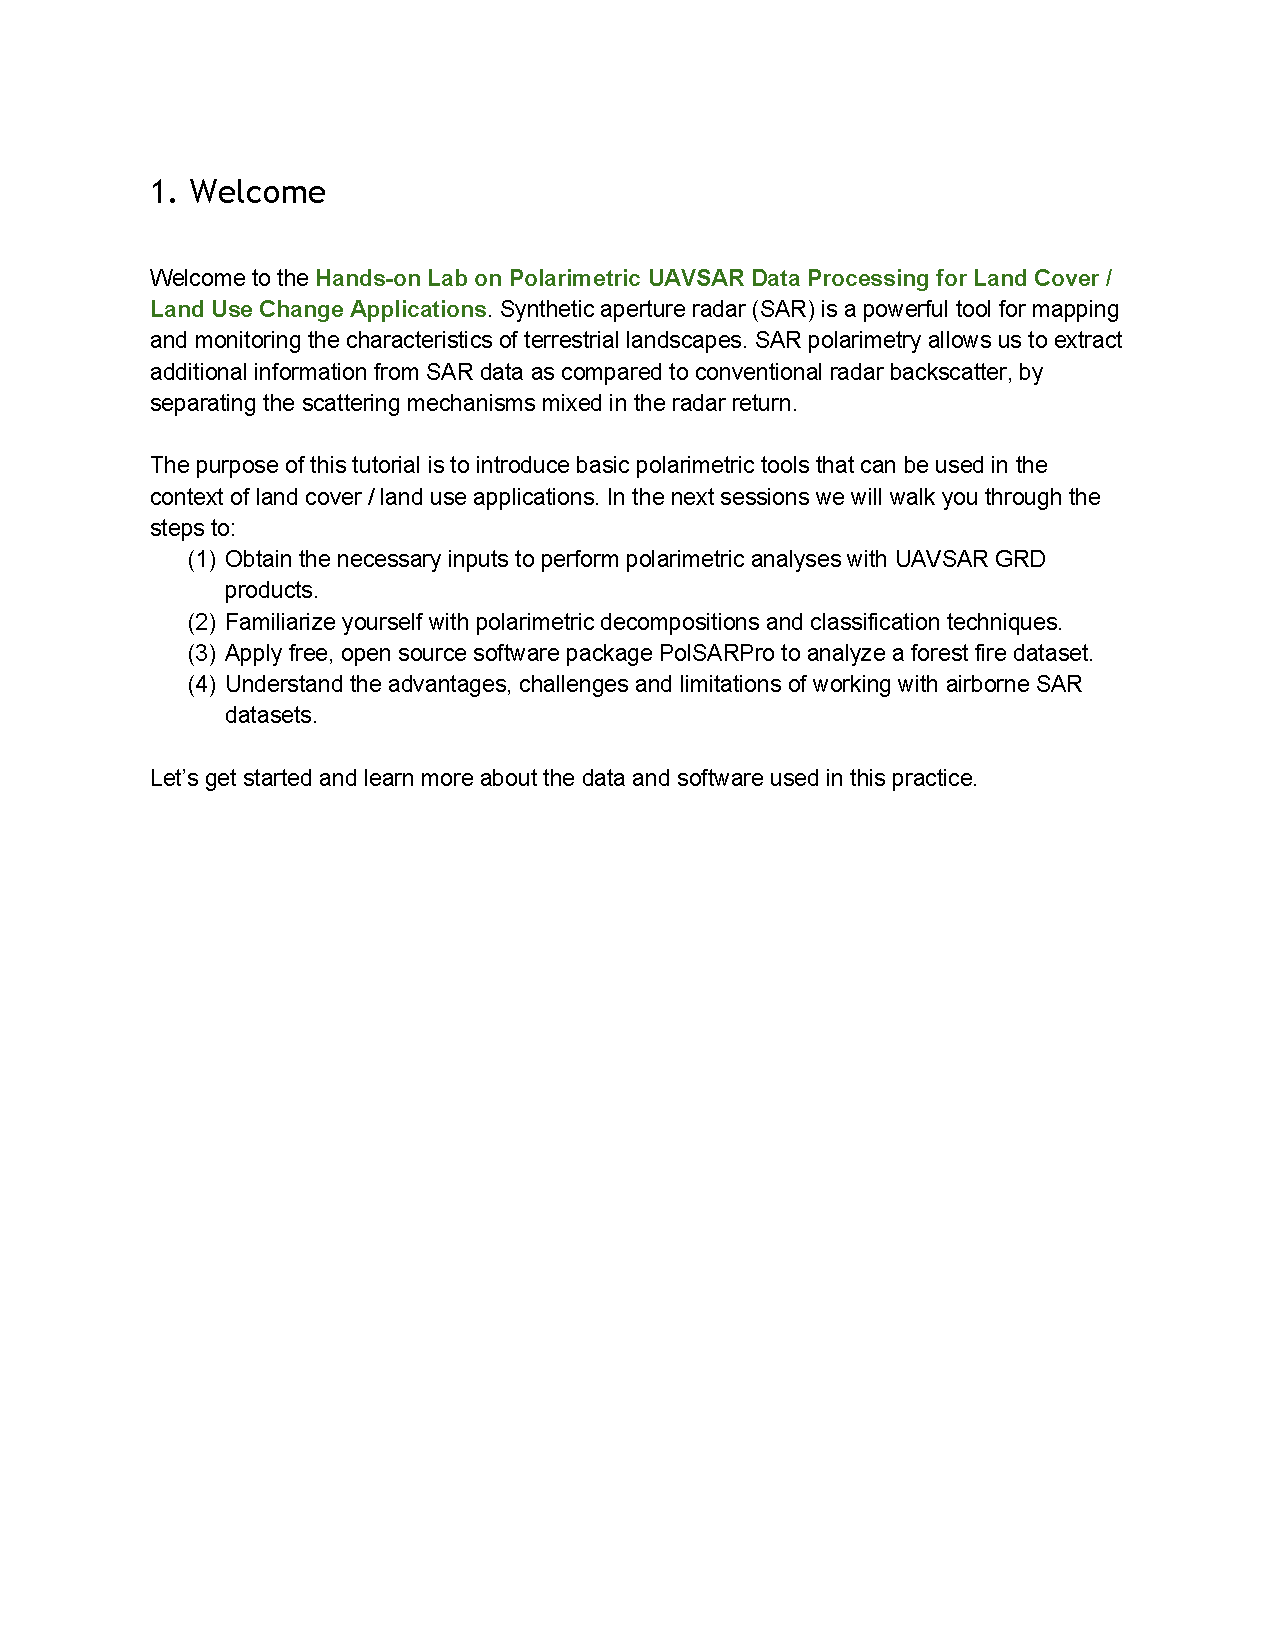
\includepdf[pages=-]{Version2Lab10Hands-onLabonPolarimetricUAVSARDataProcessingforLand-coverLand-useChangeApplications.pdf}

\chapter{Post-Processing UAVSAR Stacks With isceApp.py}
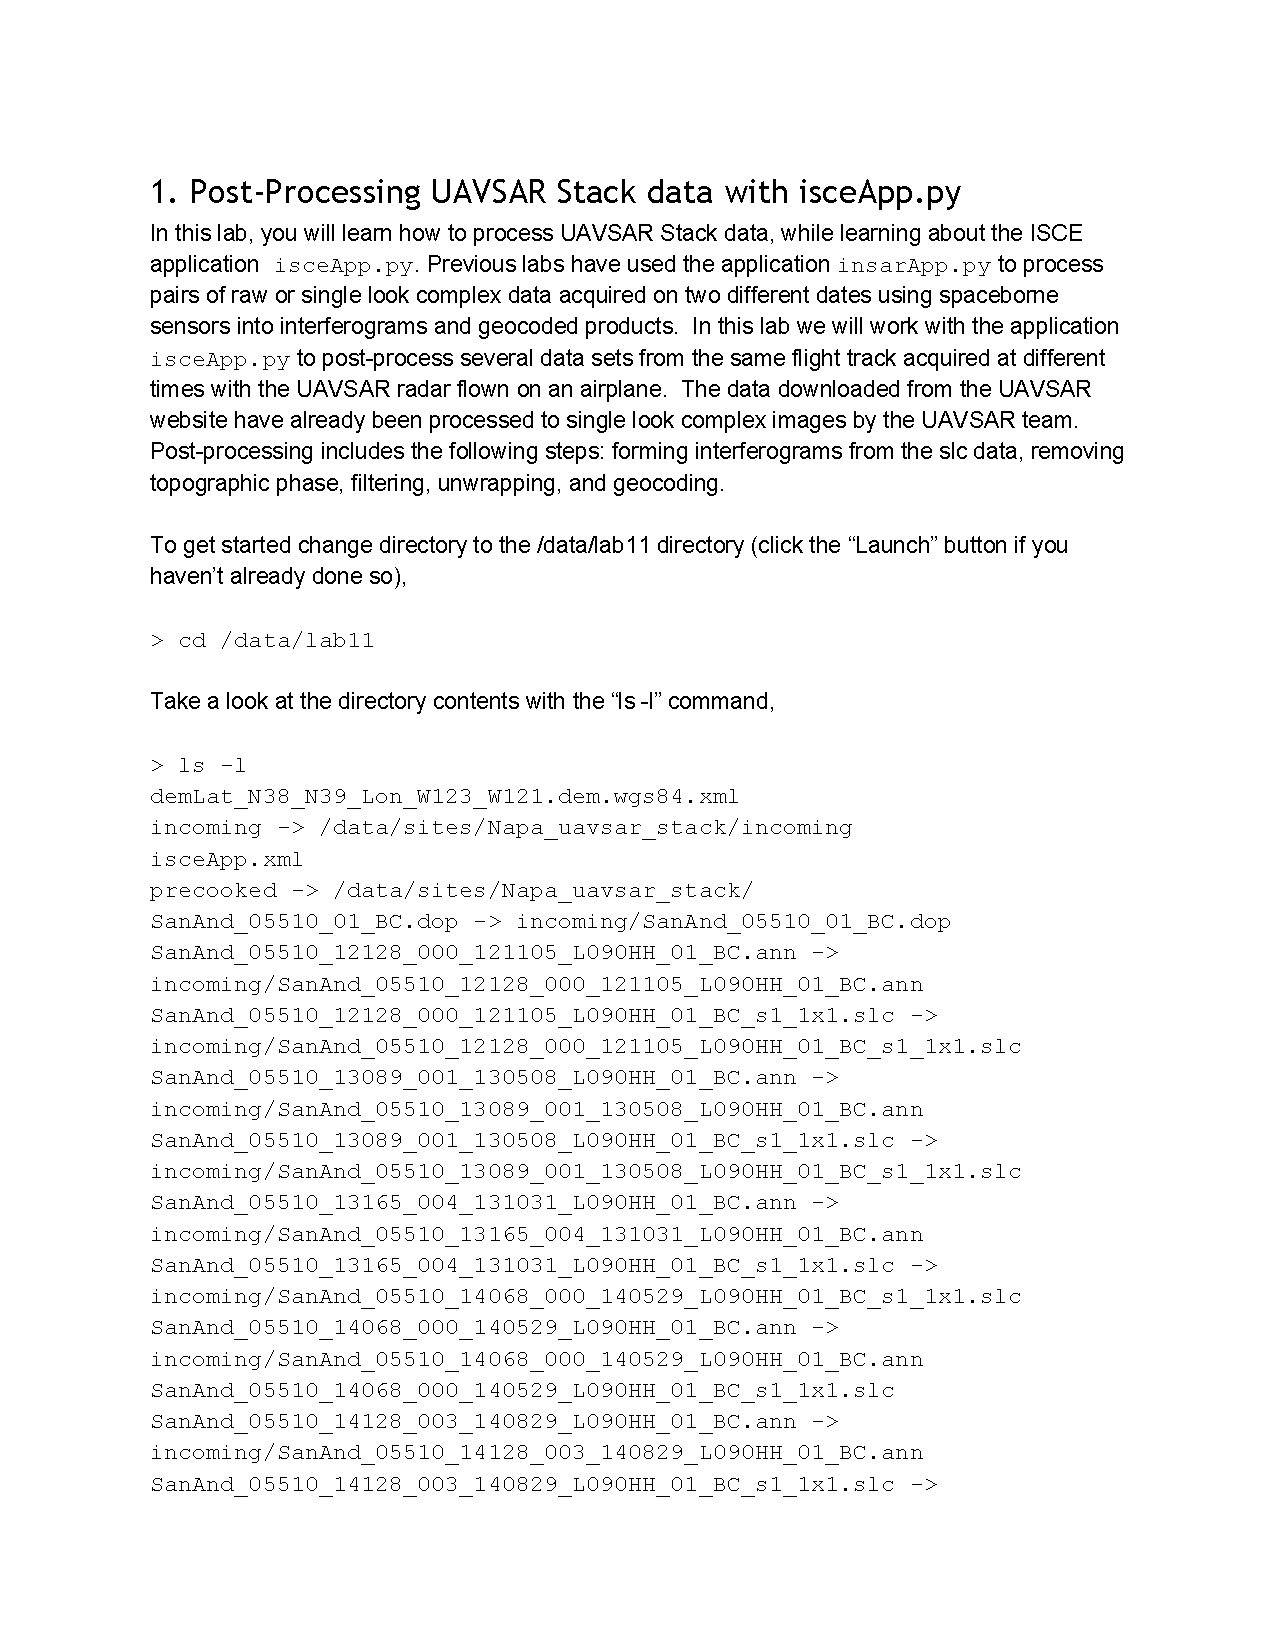
\includepdf[pages=-]{Lab11Post-ProcessingUAVSARStackswithisceApp.pdf}

\chapter{GIAnT with UAVSAR Stacks}
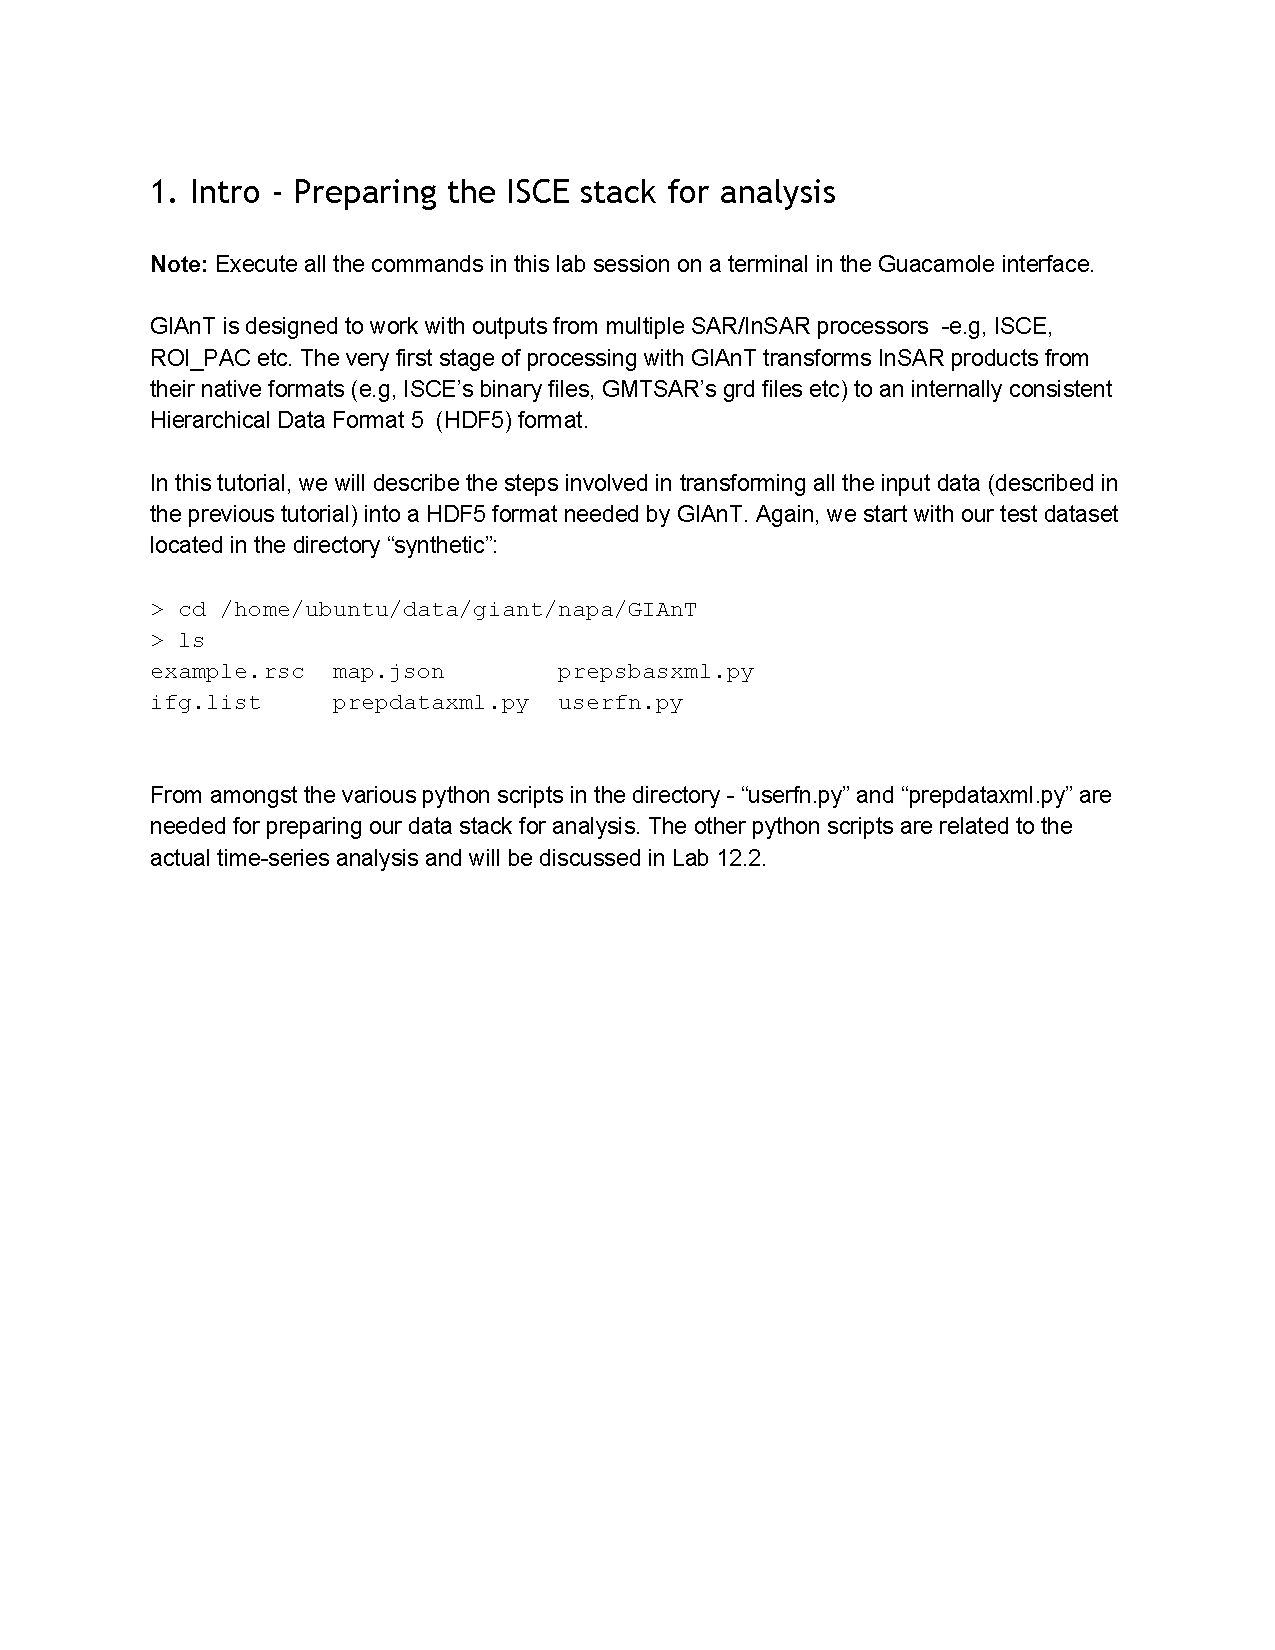
\includepdf[pages=-]{Lab12_1GIAnT_UAVSAR_reading_the_stack.pdf}
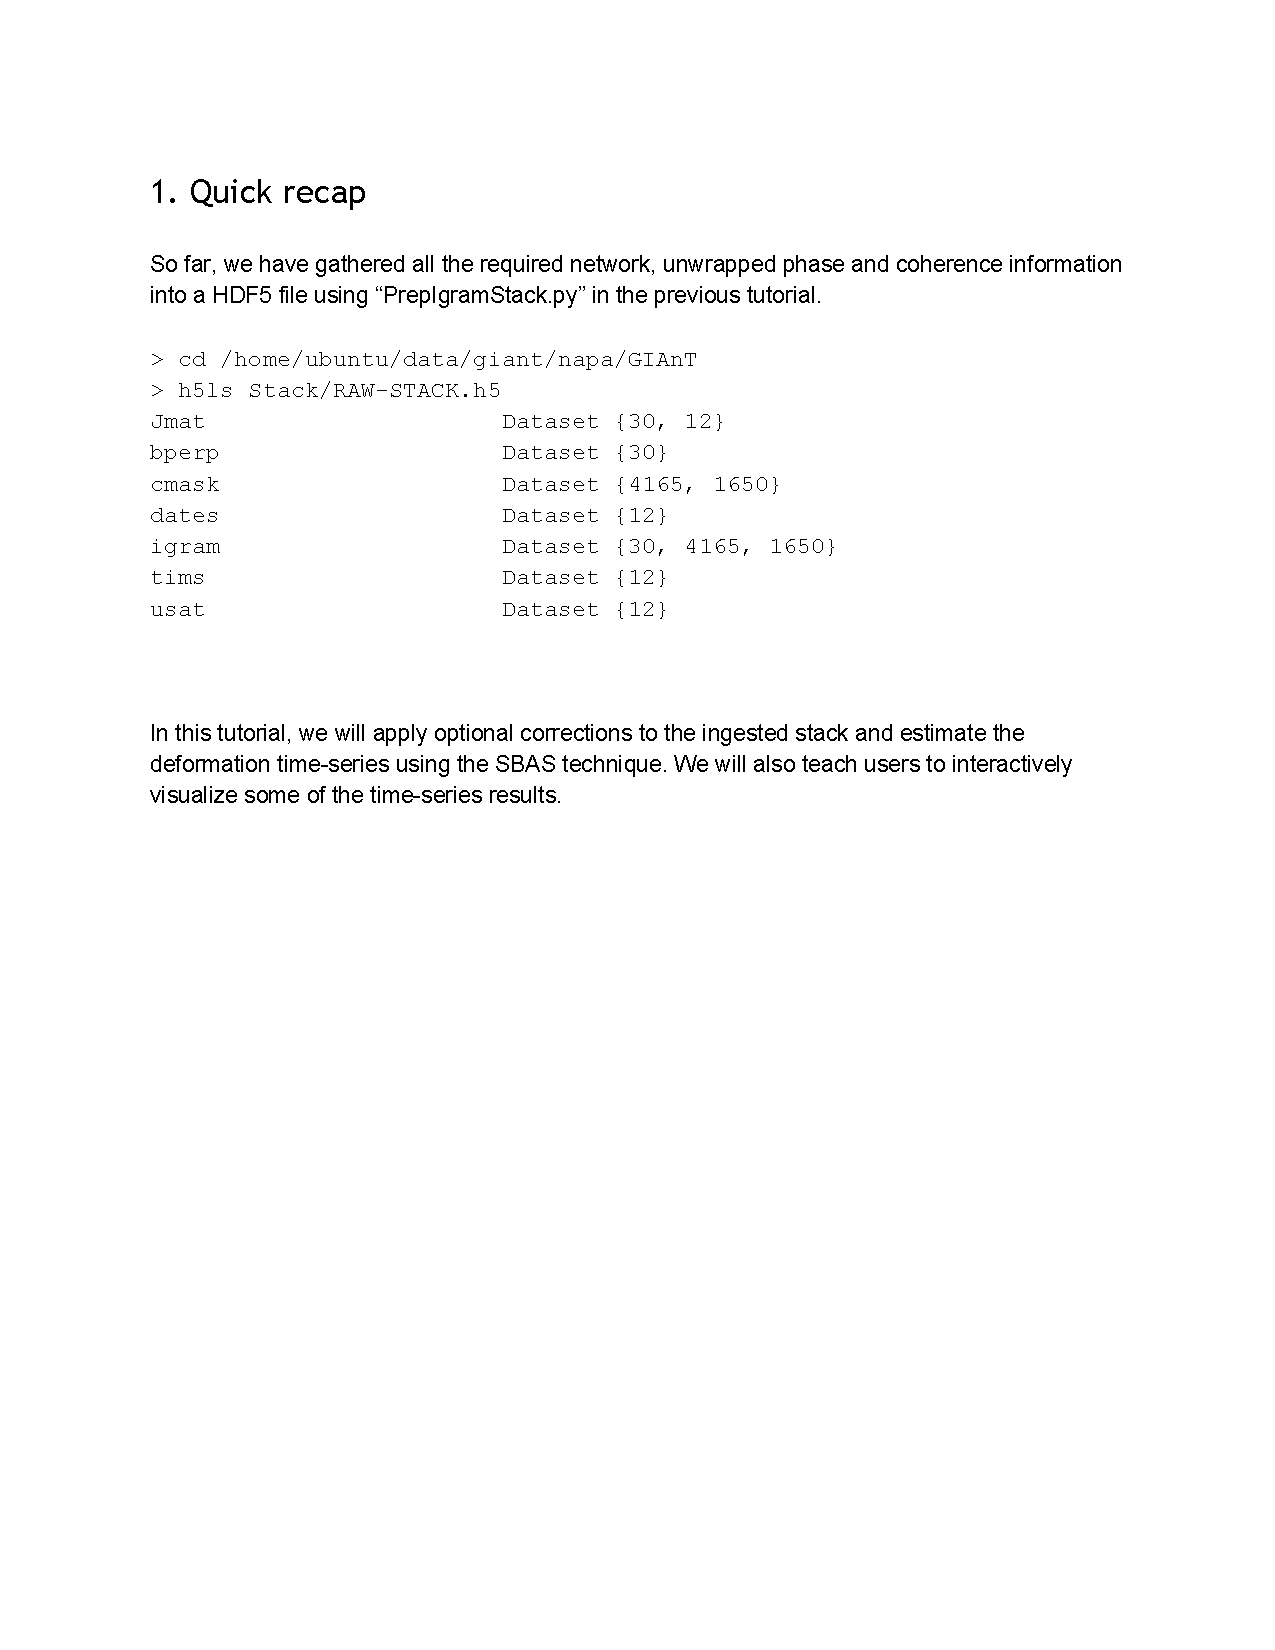
\includepdf[pages=-]{Lab12_2GIAnT_UAVSAR_inversion.pdf}


\clearpage

%\bibliography{local}
%\bibliographystyle{plain}
%\bibliographystyle{plainnat}


\end{document}
